\cotefile{57}
\scanpage{271}
- \mspage{9} -
\margin{$n^\circ\ 227$}

entiers. Le corps $k(x)$ étant une extension finie de $k(x_1,\ldots,x_r)$ le groupe des valeurs dans ce corps est aussi canoniquement isomorphe aux entiers. Donc dans le cas général, on peut aussi définir l'\uline{ordre} d'une fonction sur un diviseur premier $W$ : C'est l'entier associé à cette fonction dans le groupe des valeurs de l'anneau de valuation correspondant à $W$.

Le groupe abélien libre engendré par les diviseurs premiers de $V$ est appelé le groupe des \uline{diviseurs} de $V$. Chaque diviseur peut s'exprimer comme somme finie
\[
D=\sum n_iW_i
\]
où les $n_i$ sont des entiers $\ne 0$, et les $W_i$ sont des diviseurs premiers distincts. Le \uline{support} de $D$, i.e. l'ensemble des points dans les $W_i$, sera noté $|D|$.\margin{\uline{\unsure{$\sim W$}}} Si tous les $n_i$ sont $\geq 0$ on dira que $D$ est \uline{positif}. On voit qu'il y a une relation d'ordre partielle entre diviseurs.

Si $z$ est une fonction sur $V$, on peut lui associer le diviseur $\sum_W(\operatorname{ord}_Wz)W$, noté par $(z)$, la somme étant prise sur tous les diviseurs premiers. On sait que la fonction n'a qu'un nombre fini de zéros et de pôles, donc que cette somme est finie. Deux diviseurs $D_1$ et $D_2$ sont \uline{linéairement équivalents} s'ils diffèrent par le diviseur d'une fonction, i.e. s'il existe une fonction $z$ telle que $D_1=(z)+D_2$. Si $D$ est un diviseur, l'ensemble des diviseurs \uline{positifs} linéairement équivalents à $D$ sera noté par $\mathcal{L}(D)$. Il peut être vide. L'ensemble de tous les diviseurs linéairement équivalent à $D$ sera noté $\mathcal{L}^0(D)$.
\mspage{270}

\scanpage{272}
\uline{Questions.} \deleted{\unsure{?}} Soit $A$ un anneau local \deleted{\unsure{et}} noethérien. On suppose $A$ \uline{hensélien}, et un ``bon anneau'', i.e. $\unsure{\operatorname{Sp}}\widehat A-\unsure{\operatorname{Sp}}A$ est \deleted{\unsure{est}} un \unsure{mor!} régulier.\inserted{p. ex \deleted{\unsure{C'est}} \deleted{\unsure{un}} anneau hensélisé d'un anneau local de la géom. alg. sur $\mathbb C$} Soit $X$ propre sur $A$, et $\widehat X=X\otimes_A\widehat A$.

(i) Est-il vrai que \unsure{tte image universelle} de \unsure{--}, $\operatorname{Pic}(X_{\unsure{n}})$ \deleted{\unsure{?}} [\unsure{on a} $=:\ \unsure{\Longleftrightarrow}$ \unsure{élément} dans $\operatorname{Im}(\operatorname{Pic}(\widehat X)\mathbin{\unsure{-|\to}}\operatorname{Pic}(X_{\unsure{n}}))$] est dans $\operatorname{Im}(\operatorname{Pic}(X)\mathbin{\unsure{-|\to}}\operatorname{Pic}(X_{\unsure{n}}))$ ? En particulier, si $\widehat X/\widehat Y$ est projectif, est-il vrai que $X/Y$ est projectif ?

(ii) Supposons que $\operatorname{supp}R^1f_*(\mathcal O_X)\subset\{y\}$, \deleted{\illegible{1}} p. ex. $X|(Y-\{y\})\simeq Y-\{y\}$. Est-il vrai alors que
\[
\operatorname{Pic}(X)\xrightarrow{\sim}\operatorname{Pic}(\unsure{\widehat Y|\widehat X})\quad ??
\]
\deleted{\unsure{N.B.}}

(iii) Supposons que $Y$ soit \unsure{pt} singulier isolé en $y$. Est-il vrai que
\[
\operatorname{Pic}(Y-\{y\})\xrightarrow{\sim}\operatorname{Pic}(\widehat Y-\{\widehat y\})
\]
[Si (ii) est vrai, et si on peut désingulariser, alors (iii) est vrai\ldots.]. \unsure{Que se passe-t-il si} $y$ n'est pas isolé en $\operatorname{Sing}(Y)$, dans le cas où $A$ est un \unsure{Alg.} analytique ?
\margin{What does \unsure{Mumford's} example in ``Publications IHES'' p. 16 give ??}
\figure{\begin{tikzpicture}[x=1cm,y=1cm]
\draw[->] (2,0)..controls(-1,3)and(-.5,6)..(4.5,6.7);
\draw (2,0)..controls(1.5,-.1)and(1.5,-1)..(2.2,-1.1)--(6,-1.1)..controls(6.5,-1.1)and(6.3,-.4)..(6.8,-.4)--(10,-.4)..controls(10.6,-.3)and(10.8,.8)..(10.4,1.2)--(6.4,1.2)..controls(6.1,1.2)and(6.5,.5)..(6,.3)--(2.3,.3)..controls(2,.3)and(2,.1)..(2,0);
\draw (.4,-1.5)..controls(.6,-2.7)and(.4,-2.7)..(0,-2.9)..controls(.5,-3.1)and(.3,-4.4)..(.6,-4.5);
\end{tikzpicture}}
\mspage{271}

\scanpage{273}
- \mspage{8} -
\margin{$n^\circ\ 227$}

premier $W$ passant par $P'$, et tel que $z$ ait un zéro sur $W$. Pour le pôle, on considère $z^{-1}$ au lieu de $z$.

Nous allons maintenant étudier le groupe des valeurs associé à un diviseur premier, et montrer qu'il est canoniquement isomorphe aux entiers rationnels, ce qui nous permettra de parler de l'ordre d'un zéro ou d'un pôle d'une fonction.

L'étude étant local, on suppose que $V$ est affine. Considérons d'abord le cas où $V$ est l'espace affine $S^r$. Soit $P=(x_1,\ldots,x_r)$ un point générique de $S^r$. l'anneau $k[x]$ est factoriel, et les diviseurs premiers sont en correspondance biunivoque avec les polynômes irréductibles $p(x)=p$. Chaque fonction $z$ peut s'écrire
\[
z=p^mR(x)
\]
où $R(x)$ est une fonction rationnelle dont le numérateur et le dénominateur sont premiers à $p$. Alors $z$ a un zéro ou un pôle sur $W$ selon que $m>0$ ou $m<0$. On voit que le groupe des valeurs est canoniquement isomorphe aux entiers, et on note
\[
m=\operatorname{ord}_W z.
\]
C'est l'\uline{ordre} de la fonction $z$ sur $W$. Dans le premier cas, $z$ a un zéro d'ordre $m$, et dans le second, un pôle d'ordre $m$.

Passons au cas général, avec un point générique $(x_1,\ldots,x_n)$ de $V$. Soit $(x')$ un point générique d'un diviseur premier $W$ de $V$. On peut supposer $x'_1,\ldots,x'_{r-1}$ algébriquement indépendant. Soit $x_r$ indépendant de $x_1,\ldots,x_{r-1}$. Alors la place qui induit $(x)\longrightarrow(x')$ induit une place sur le sous corps $k(x_1,\ldots,x_r)$ et peut être considérée comme induisant un diviseur premier sur l'espace affine $S^r$. On a vu plus haut que le groupe des valeurs sur ce sous corps est isomorphe aux
\mspage{272}

\scanpage{274}
\unsure{Polarisation|Polarisations}

Schémas de Néron-\unsure{Sévéri|Séveri}
\mspage{273}

\scanpage{275}
\uline{Définition} $X$ préschéma sur $S$. Un élément $\xi$ de $\operatorname{Pic}(X/S)$ est dit \uline{numériquement équivalent à $0$} si sa restriction à tte fibre $X_s$ est numériquement \unsure{équivalent} à zéro [ie. un multiple d'icelle peut se déformer dans $0$]. Deux \unsure{éléme} $\xi,\xi'$ de $\operatorname{Pic}(X/S)$ sont dits numériquement équivalents si $\xi-\xi'$ est numériquement équivalent à $0$,

Soit $\operatorname{Pic}^{\tau}(X/S)\subset\operatorname{Pic}^{\deleted{\unsure{\tau}}}(X/S)$ des $\xi$ numériquement \unsure{équivalts} à $0$, et $\deleted{\unsure{\operatorname{Pol}}}\inserted{\unsure{\operatorname{N\acute{e}r}}}'(X/S)=\operatorname{Pic}(X/S)/\operatorname{Pic}^{\tau}(X/S)$. Noter : si \deleted{$S'\to S$ est fid plat [et \unsure{qu. cpt}] et} $S'\to S$ est un \unsure{changt} de base, alors $\operatorname{Pic}(X/S)\to\operatorname{Pic}(X'/S')$ induit $\operatorname{Pic}^{\tau}(X/S)\to\operatorname{Pic}^{\tau}(X'/S')$, et si $S'\to S$ est surjectif, alors \deleted{un élément $\xi$ de} $\operatorname{Pic}^{\tau}(X/S)$ est exactement l'image inverse de $\operatorname{Pic}^{\tau}(X'/S')$ par $\operatorname{Pic}^{\deleted{\unsure{\tau}}}(X/S)\to\operatorname{Pic}(X'/S')$, donc dans ce cas
\[
\deleted{\unsure{\operatorname{Pol}}}\inserted{\unsure{\operatorname{N\acute{e}r}}}'(X/S)\longrightarrow\deleted{\unsure{\operatorname{Pol}}}\inserted{\unsure{\operatorname{N\acute{e}r}}}'(X'/S')\quad\text{est \uline{injectif}}
\]
\margin{\diagram{\begin{tikzcd}X\arrow[d]&X'\arrow[l]\arrow[d]\\S&S'\arrow[l]\end{tikzcd}}}

Considérons $S'\mapsto\operatorname{Pol}'(X'/S')$ comme foncteur contravariant $(\operatorname{Sch})^0_{/S}\longrightarrow(\operatorname{Ens})$, et \uline{rendons le exact pour les morphismes fid plats \deleted{\unsure{qu. cpts}} \inserted{loc. de type} fini} [donc pour la localisation habituelle aussi]. On trouve un foncteur $S'\mapsto\deleted{\unsure{\operatorname{Pol}}}\inserted{\unsure{\operatorname{N\acute{e}r}}}(X'/S')$, et en particulier on a un \inserted{ens} $\deleted{\unsure{\operatorname{Pol}}}\inserted{\unsure{\operatorname{N\acute{e}r}}}(X/S)$, ens des polarisations de $X$ sur $S$.
\mspage{274}

\scanpage{276}
Interprétation lorsque $\uline{\operatorname{Pic}}_{X/S}$ existe, ($\uline{\operatorname{Pic}}^{\tau}_{X/S}$ ouvert !)

Alors la donnée d'un \unsure{élémt} de $\uline{\operatorname{Pol}}'(X/S)$\deleted{$\unsure{X/S}$} équivaut à la donnée d'un sous-préschéma \inserted{\uline{ouvert}} $P$ de $\uline{\operatorname{Pic}}^{\tau}_{X/S}$ qui soit un fibré principal homogène \uline{trivial} sous $\uline{\operatorname{Pic}}^{\tau}_{X/S}$. Alors $\deleted{\unsure{\operatorname{Pol}}}\inserted{\operatorname{N\acute{e}r}}(X/S)$ est l'ensemble des sous-préschémas \deleted{ouverts} de $\uline{\operatorname{Pic}}_{X/S}\deleted{(X/S)}$ qui sont formellement principaux homogènes $P$ sous $\uline{\operatorname{Pic}}^{\tau}_{X/S}$, et sont trivialisés par une extension fid plate loc. de type fini. [N.B. \deleted{lorsque}\inserted{Ces} sous-préschémas sont nécessairement \uline{ouverts}. Si $\uline{\operatorname{Pic}}^{\tau}_{X/S}$ est plat et de type fini sur $S$, alors la condition supplémentaire sur $P$ qu'on vient de mettre signifie aussi que $P$ est \uline{fid plat} et de type fini sur $S$]. Par suite,

\deleted{dire que lorsque}

\uline{Proposition} \uline{Supposons que $\uline{\operatorname{Pic}}_{X/S}$ existe, et que $\uline{\operatorname{Pic}}^{\tau}_{X/S}$ soit fid plat [de type fini] sur $S$}. Pour que le foncteur $\uuline{\deleted{\unsure{\operatorname{Pol}}}\inserted{\operatorname{N\acute{e}r}}}_{X/S}$ dans \deleted{$\unsure{(\operatorname{Ens})}$} $(\operatorname{Sch})^0_{/S}$ soit représentable, il f. et s. que le quotient $\uline{\deleted{\unsure{\operatorname{Pol}}}\inserted{\operatorname{N\acute{e}r}}}_{X/S}=\uline{\operatorname{Pic}}^{\deleted{\unsure{\tau}}}_{X/S}/\uline{\operatorname{Pic}}^{\tau}_{X/S}$ existe, et \deleted{alors} que $\uline{\operatorname{Pic}}_{X/S}\to\uline{\operatorname{N\acute{e}r}}_{X/S}$ soit \uline{fid plat \deleted{et \unsure{qu. cpt}} \inserted{et de type fini} de noyau $\uline{\operatorname{Pic}}^{\tau}_{X/S}$}
\margin{de type fini inutile ?}
\figure{\begin{tikzpicture}\draw(0,0)--(0,4.6);\end{tikzpicture}}
\mspage{275}

\scanpage{277}
et alors $\uuline{\operatorname{N\acute{e}r}}_{X/S}$ est représenté par $\uline{\operatorname{N\acute{e}r}}_{X/S}$

\uline{Corollaire 1} S'il en est ainsi, $\uline{\operatorname{N\acute{e}r}}^{\deleted{\unsure{\tau}}}_{X/S}$ est \deleted{\unsure{représentable}} séparé ssi $\uline{\operatorname{Pic}}^{\tau}_{X/S}$ est fermé dans $\uline{\operatorname{Pic}}_{X/S}$. En tous cas, $\uline{\operatorname{N\acute{e}r}}_{X/S}$ est \uline{non ramifié} sur $S$.

\uline{Corollaire 2} Supposons que $\uline{\operatorname{Pic}}^{\tau}_{X/S}$ soit \uline{propre} \inserted{et \uline{plat}} sur $S$, et que $\uline{\operatorname{Pic}}^{\deleted{\unsure{\tau}}}_{X/S}$ soit réunion \inserted{croissante} d'ouverts \inserted{$U_i$} stables par $\uline{\operatorname{Pic}}^{\tau}_{X/S}$ et quasi-projectifs sur $S$. [cette dernière condition est conséquence de $\uline{\operatorname{Pic}}^{\tau}_{X/S}$ de type fini sur $S$, dans le cas où $X$ est projectif, plat,\inserted{\deleted{\unsure{plat et}} $\unsure{f_*(\mathcal O_X)=\mathcal O_S}$ universellement} et primaire sur $S$]. Alors $\uline{\operatorname{N\acute{e}r}}_{X/S}$ existe et est séparé non ramifié sur $S$.
\margin{La première condition est vérifiée si les fibres de $X/S$ ont des \unsure{Nér géo} sans torsion et des $\operatorname{Pic}^0$ propres\ldots}

Il semble que dès que $\uline{\operatorname{Pic}}^{\tau}_{X/S}$ est \uline{plat} \deleted{\unsure{sur}} sur $S$\inserted{et fermé dans $\uline{\operatorname{Pic}}_{X/S}$}, $\uline{\operatorname{N\acute{e}r}}_{X/S}$ doive exister : c'est lié à la question de la caractérisation des foncteurs représentés par un objet non ramifié sur $S$\ldots. Au concours ! [A vrai dire, même l'existence de $\uline{\operatorname{Pic}}^{\deleted{\unsure{\tau}}}_{X/S}$ ne semble pas indispensable !]
\margin{?}
\figure{\begin{tikzpicture}[x=1cm,y=1cm]
\draw (0,7)--(0.02,6.15); \draw (0.12,5)--(0.13,2.25); \draw (0.08,1.25)--(0,0.65)--(0.12,-0.45);
\draw (2.5,3.12)..controls (2.1,3.5) and (4.4,3.4)..(4.85,3.35)..controls (5.1,3.1) and (4.8,3.0)..(4.6,3.0)--(2.6,2.94)--(2.55,2.65);
\draw (1.1,1.4)..controls (0.7,1.7) and (2.5,1.75)..(2.8,1.5)--(2.8,1.25)--(1.2,1.16)--(1.15,0.98);
\end{tikzpicture}}
\mspage{276}

\scanpage{279}
\uline{Schémas polarisés}

Soit $X$ projectif sur $S$ loc. noeth., \inserted{plat et Steinien,}\deleted{\unsure{Noter qu'une} \uline{polarisation stricte} de $X$ est la donnée d'un élément de \deleted{$\unsure{\operatorname{Pic}(X/S)}$} $\operatorname{Pic}(X)$, \deleted{\illegible{1}}\inserted{\unsure{no.}} qui induit sur chaque fibre de $X/S$ un faisceau inversible \unsure{qui est} \illegible{2}}
\margin{semble excessif, par exemple pour l'énoncé du th. de Matsusaka}
\margin{\deleted{\unsure{défini par} \illegible{2} \unsure{inversible} \illegible{2} $X/S$}}

On suppose que $\uuline{\operatorname{Pic}}_{X/S}$ existe. Soit $\deleted{\unsure{\operatorname{Pol}}}\inserted{\operatorname{N\acute{e}r}}'(\unsure{X'|X}/S)$ l'ensemble quotient de $\operatorname{Pic}(X)^{\deleted{\unsure{X/S}}}$ \deleted{$\unsure{0}$} par $\operatorname{Pic}^{\deleted{\unsure{\tau}}}(X)^{\tau/S}$, où $\operatorname{Pic}(X)^{\tau/S}$ est l'image inverse de $\Gamma(S,\uuline{\operatorname{Pic}}^{\tau}_{X/S})$ par $\operatorname{Pic}(X)\to\Gamma(S,\uuline{\operatorname{Pic}}_{X/S})$. Les éléments de $\operatorname{N\acute{e}r}'(X/S)$ s'appellent \deleted{\unsure{pseudo}\uline{polarisations}}\inserted{\unsure{néronisations}} \uline{strictes}. On pose $\uline{\deleted{\unsure{\operatorname{Pol}}}\inserted{\operatorname{N\acute{e}r}}}'_{X/S}(T)=\deleted{\unsure{\operatorname{Pol}}}\inserted{\operatorname{N\acute{e}r}}'(X_T/T)$, c'est un foncteur contravariant en $T$, soit $\uline{\deleted{\unsure{\operatorname{Pol}}}\inserted{\operatorname{N\acute{e}r}}}'_{X/S}$, \deleted{multiplicatif} \unsure{donc} \illegible{1} \deleted{est} \unsure{au moins un préfaisceau}, $\rho$
\margin{$\rho$ et tel que pour $T'\to T$ fid plat de type fini, $\uline{\deleted{\unsure{\operatorname{Pol}}}\inserted{\operatorname{N\acute{e}r}}}'_{X/S}(T)\to\uline{\deleted{\unsure{\operatorname{Pol}}}\inserted{\operatorname{N\acute{e}r}}}'_{X/S}(T')$ soit injectif [i.e. les morphismes fid plats de type fini sont de descente pour $\uline{\operatorname{Pol}}'_{X/S}$]}

Rendons ce foncteur compatible avec la descente fid plate de type fini, on trouve un foncteur $\uline{\deleted{\unsure{\operatorname{Pol}}}\inserted{\operatorname{N\acute{e}r}}}^{\deleted{\unsure{\tau}}\prime\prime}_{X/S}$. \deleted{Un élément de} \unsure{On pose} $\uline{\deleted{\unsure{\operatorname{Pol}}}\inserted{\operatorname{N\acute{e}r}}}''_{X/S}(S)=\deleted{\unsure{\operatorname{Pol}}}\inserted{\operatorname{N\acute{e}r}}''(X/S)$, les éléments de cet ensemble s'appellent les \deleted{\unsure{pseudo}\uline{prépolarisations}}\inserted{\unsure{néronisations}} \uline{de $X$ sur $S$}. Donc :
\[
\text{(a)}\quad\uline{\deleted{\unsure{\operatorname{Pol}}}\inserted{\operatorname{N\acute{e}r}}}''_{X/S}(T)\simeq\deleted{\unsure{\operatorname{Pol}}}\inserted{\operatorname{N\acute{e}r}}''(X_T/T)\quad\text{(isom can)},
\]
une prépolarisation de $X/S$ est définie par la donnée d'une polarisation stricte $\xi$ d'un $X_T/T$,\inserted{i.e. d'un $\uline{L}$ inversible \deleted{\unsure{rel. ample}} sur $X_T/T$,} où $T$ est fid plt de type fini sur $S$, tel que les deux images inverses de $\xi$ sur $X_{T\times_S T}/T\times_S T$ soient identiques, i.e. tel $L$ \unsure{que} $p_1^*(\uline{L})p_2^*(\uline{L})^{-1}$ soit de \deleted{torsion}\inserted{\unsure{équiv. à $0$}} \unsure{rel.} à $T\times_S T$.
\figure{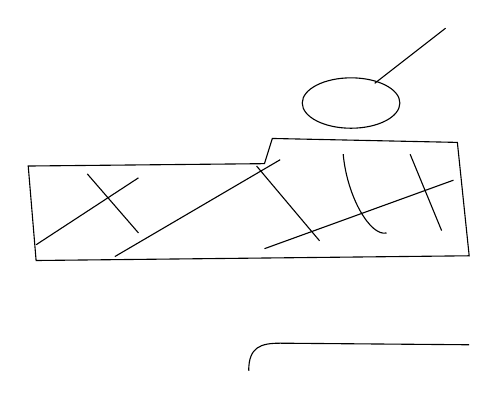
\begin{tikzpicture}[x=1cm,y=1cm]
\draw (4.1,3.7) ellipse (0.62 and 0.32); \draw (4.4,3.95)--(5.3,4.65);
\draw (0,2.9)--(0.1,1.7)--(5.6,1.76)--(5.45,3.2)--(3.1,3.25)--(3.0,2.93)--cycle;
\draw (0.1,1.9)--(1.4,2.75) (0.75,2.8)--(1.4,2.05) (1.1,1.75)--(3.2,2.98) (2.9,2.9)--(3.7,1.95) (3,1.85)--(5.4,2.72) (4,3.05)..controls (4.05,2.5) and (4.35,2)..(4.55,2.05) (4.85,3.05)--(5.25,2.08);
\draw (3.2,0.65)--(5.6,0.63); \draw (3.2,0.65)..controls (2.95,0.65) and (2.8,0.6)..(2.8,0.3);
\end{tikzpicture}}
\mspage{278}

\scanpage{280}
$\xi$ de $\uline{\deleted{\unsure{\operatorname{Pol}}}\inserted{\operatorname{N\acute{e}r}}}'(X_T/T)$ et $\xi'$ de $\uline{\deleted{\unsure{\operatorname{Pol}}}\inserted{\operatorname{N\acute{e}r}}}'(X_{T'}/T')$ définissent la $\unsure{=}$ prépolarisation sss leurs images inverses dans $\uline{\deleted{\unsure{\operatorname{Pol}}}\inserted{\operatorname{N\acute{e}r}}}'(X_{T\times_S T'}/T\times_S T')$ sont égales, i.e. si \unsure{l'i} $p_1(\uline{L})p_2(\uline{L}')^{-1}$ est \deleted{\unsure{torsion.}} équivalent à $0$ rel. à $T\times_S T'$.

Si p. ex. $\uuline{\operatorname{Pic}}^{\tau}_{X/S}$ est plat sur $S$ et si le quotient $\inserted{\uuline{\deleted{\unsure{\operatorname{Pol}}}\inserted{\operatorname{N\acute{e}r}}}_{X/S}}\ \uuline{\operatorname{Pic}}_{X/S}/\uuline{\operatorname{Pic}}^{\tau}_{X/S}$ existe ``raisonnablement'' [i.e. le \deleted{\unsure{grp}} \unsure{graphe} d'équivalence défini par $\uuline{\operatorname{Pic}}^{\tau}_{X/S}$ est effectif, et la projection $\uuline{\operatorname{Pic}}_{X/S}\to\uuline{\operatorname{Pic}}_{X/S}/\uuline{\operatorname{Pic}}^{\tau}_{X/S}$ fid plate] -- p. ex. si $\uuline{\operatorname{Pic}}^{\tau}_{X/S}$ est \uline{propre} sur $S$ -- alors \deleted{\unsure{on prouve}} $\uline{\deleted{\unsure{\operatorname{Pol}}}\inserted{\operatorname{N\acute{e}r}}}''_{X/S}$ s'identifie au foncteur associé à \deleted{\unsure{Alors}} $\uuline{\operatorname{N\acute{e}r}}_{X/S}$, donc les néronisations de $X/S$ sont les sections de $\uuline{\operatorname{N\acute{e}r}}_{X/S}$ sur $S$, ce qui justifie la terminologie et \deleted{\unsure{en outre}} la notation

\deleted{Deux}
\deleted{Deux néronisations sont dites \uline{équivalentes} si (on appelle néronisation)}

On définit un ss-ensemble $\operatorname{N\acute{e}r}'{}^+(X/S)$ de $\operatorname{N\acute{e}r}'(X/S)$ par les classes de faisceaux inv. sur $X$ \deleted{\unsure{abs}} amples rel. à $S$, d'où un ss-foncteur $\uline{\operatorname{N\acute{e}r}}^{\unsure{+}\prime}_{X/S}$, donnant naissance à un ss-foncteur $\uline{\operatorname{N\acute{e}r}}^{+\prime\prime}_{X/S}$ de $\uline{\operatorname{N\acute{e}r}}''_{X/S}$, qui s'explicite en remplaçant ci-dessus les ``faisceaux inversibles'' par ``faisceaux inversibles rel! amples''. Dans le cas particulier
\mspage{279}

\scanpage{281}
envisagé où le schéma de Néron $\uuline{\operatorname{N\acute{e}r}}_{X/S}$ existe, le foncteur $\uline{\operatorname{N\acute{e}r}}^{+\prime\prime}_{X/S}$ est associé au sous-schéma ouvert induit $\uuline{\operatorname{N\acute{e}r}}^{+}_{X/S}$ de $\uuline{\operatorname{N\acute{e}r}}_{X/S}$, image de $\uuline{\operatorname{Pic}}^{+}_{X/S}$. Un élément de $\uline{\operatorname{N\acute{e}r}}^{+\prime\prime}_{X/S}(S)=\operatorname{N\acute{e}r}^{+\prime\prime}(X/S)$ est appelé une \uline{polarisation} \deleted{\unsure{positive}} de $X/S$. Elles \inserted{forment un pré-monoïde (sans élément neutre) commutatif}\inserted{\unsure{plongé dans le groupe} $\uline{\operatorname{N\acute{e}r}}''(X/S)$}.

Deux polarisations $\xi,\xi'$ sont dites \uline{équivalentes} s'il existe des entiers $n,n'>0$ tels que $n\xi=n'\xi'$. Les \inserted{classes de} polarisations correspondent donc aux demi-droites d'un cône convexe $C$ \deleted{[ouvert]} dans un espace vectoriel $V$ sur $\unsure{\mathbb Q|\mathbf Q}$ engendré par $C$, dont les pts de $C$ sont ``\unsure{intérieurs}'' \unsure{---}.

Polarisation \uline{très ample} (pour une polarisation donnée, il en existe tjrs une équivalente qui est \uline{très ample})
\figure{\begin{tikzpicture}[x=1cm,y=1cm]
\draw (0,0.4)..controls (0.1,0.8) and (0.4,0.95)..(0.65,1.05); \draw (0.65,1.05)..controls (0.4,1.1) and (0.4,1.25)..(0.35,1.5);
\draw (2,0)--(2,0.3)..controls (2.0,0.48) and (2.2,0.52)..(2.45,0.52)--(3.45,0.55);
\end{tikzpicture}}
\mspage{280}

\scanpage{282}
Exemples
\mspage{281}

\scanpage{283}
\margin{\figure{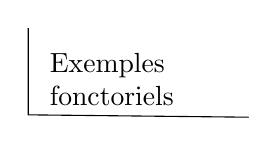
\begin{tikzpicture}\node[align=left,anchor=west] at (0.15,0.45) {\unsure{Exemples}\\fonctoriels};\draw (0,1.1)--(0,0)--(2.8,-0.03);\end{tikzpicture}}}

\diagram{\begin{tikzcd}X\arrow[d,"g"]\\Y\arrow[d,"f"]\\S\end{tikzcd}}

\diagram{\begin{tikzcd}[column sep=small]
&&&\Gamma(\deleted{\unsure{Y,}}\uuline{\operatorname{Pic}}_{X/Y}\unsure{,|/}Y)\arrow[d,equal]\\
0\arrow[r]&\operatorname{Pic}(Y)\arrow[r]&\operatorname{Pic}(X)\arrow[r]&\operatorname{Pic}(X/Y)
\end{tikzcd}}
\deleted{$\unsure{\Gamma(S,\prod_{Y/S}\uline{\operatorname{Pic}})}$}
\margin{surjectif si $X/Y$ a une section}

Pourvu que $g$ soit qu. cpt séparé et $\mathcal O_Y\overset{\sim}{\longrightarrow}g_*(\mathcal O_X)$.

-- Si cette dernière condition est $S$-universelle, alors \deleted{pour} faisant un changement de base quelconque $S'\longrightarrow S$, et passant aux ``faisceaux'' associés dans la suite exacte de \deleted{foncteurs} ``préfaisceaux'' ainsi obtenue, on trouve une suite exacte
\diagram{\begin{tikzcd}
0\arrow[r]&\uuline{\operatorname{Pic}}_{Y/S}\arrow[r]&\uuline{\operatorname{Pic}}_{X/S}\arrow[r]&\prod_{Y/S}\uuline{\operatorname{Pic}}_{X/Y}
\end{tikzcd}},
avec d'ailleurs un zéro à droite \inserted{\unsure{et splitting}} si $X/Y$ a une section. Donc si les foncteurs envisagés sont représentables, on trouve une suite \uline{exacte}
\diagram{\begin{tikzcd}
0\arrow[r]&\uline{\operatorname{Pic}}_{Y/S}\arrow[r]&\uline{\operatorname{Pic}}_{X/S}\arrow[r]&\prod_{Y/S}\uline{\operatorname{Pic}}_{X/Y}
\end{tikzcd}}
où la dernière flèche a un inverse à droite si $X/Y$ a une section. Dans ce cas, ceci donne un isom
\[
\uline{\operatorname{Pic}}_{X/S}\simeq\uline{\operatorname{Pic}}_{Y/S}\times\prod_{Y/S}\uline{\operatorname{Pic}}_{X/Y}
\]
[ceci généralise la relation connue, quand $X=Y\times_S Z$, $Z$ muni d'une section sur $S$
\[
\uline{\operatorname{Pic}}_{X/S}\simeq\uline{\operatorname{Pic}}_{Y/S}\times\uline{\operatorname{Pic}}_{Z/S}\times\uline{\operatorname{Hom}}_{\text{pointé}}(Y,\uline{\operatorname{Pic}}^{\unsure{\tau|0}}_{Z/S})
\]
]
\mspage{282}

\scanpage{284}
Soit $S$ un préschéma de base, $A$ un schéma abélien sur $S$, $B$ un schéma sur $S$, $\Gamma$ un groupe fini, opérant sur $A$ par automorphismes et sur $B$ sans pt fixe, alors $\Gamma$ opère sur $A\times B$ diagonalement, et on peut considérer $X=(A\times B)/\Gamma$ comme un préschéma \deleted{sur} \uline{abélien} sur $Y=B/\Gamma$. On a donc, si \deleted{\unsure{on suppose que}} comme $X/Y$ \deleted{est} a une section,
\[
\uuline{\operatorname{Pic}}_{X/S}\simeq\uuline{\operatorname{Pic}}_{Y/S}\times\prod_{Y/S}\uuline{\operatorname{Pic}}_{X/Y}
\]
\margin{\diagram{\begin{tikzcd}[column sep=small,row sep=small]
X\arrow[d,"f"']&A\times_S B\arrow[l,"\Gamma"']\arrow[d,"\unsure{\mathrm{pr}_1}"]\\
Y\arrow[d,"g"']&B\arrow[l,"\Gamma"]\arrow[dl,no head]\\S&
\end{tikzcd}}}
donc, si \inserted{$B\longrightarrow S$ donc} $g$ est disons projectif et simple, et $A\longrightarrow S$ projectif, on aura
\[
\uline{\operatorname{Pic}}_{X/S}\simeq\uline{\operatorname{Pic}}_{Y/S}\times\prod_{Y/S}\uline{\operatorname{Pic}}_{X/Y}
\]
Or on a
\[
\prod_{Y/S}\uuline{\operatorname{Pic}}_{X/Y}\simeq
\inserted{\prod_{Y/S}(A'\times B)/\Gamma\simeq}
\uuline{\operatorname{Hom}}_{S,\Gamma}(B,\uline{\operatorname{Pic}}_{A/S})
\]
\inserted{\uline{Soit}} $A'$ est le schéma abélien dual de $A$, sur lequel on fait opérer $\Gamma$ par ``transport de structure'';
\margin{et $\uline{N}$ le schéma de Néron-\unsure{Sévéri}. On a une suite exacte
\diagram{\begin{tikzcd}[column sep=small]
0\arrow[r]&\uuline{\operatorname{Hom}}_{S,\Gamma}(B,A')\arrow[r]&\uuline{\operatorname{Hom}}_{S,\Gamma}(B,\uline{\operatorname{Pic}}_{A/S})\arrow[r]&\uuline{\operatorname{Hom}}_{S,\Gamma}(B,\uline{\operatorname{NS}}_{A/S})\arrow[d,equal]\\&&&\uuline{N}^{\Gamma}
\end{tikzcd}}
d'où
\[
\uuline{\operatorname{Pic}}_{X/S}^{\tau}\simeq\uuline{\operatorname{Pic}}_{Y/S}^{\tau}\times\uuline{\operatorname{Hom}}_{S,\Gamma}(B,A')^{\tau}
\]
}
\uline{Si} $A'^{\Gamma}$ \uline{est} \unsure{---} \uline{à fibres discrètes} sur $S$ [c'est le cas si parmi les opérations de $\Gamma$ il y a la symétrie $x\mapsto -x$] \inserted{\uline{si $B$ un} schéma abélien, sur lequel} \deleted{\unsure{le groupe} \unsure{qui}\illegible{3}} \inserted{\unsure{opère par translations}}, on voit facilement que
\[
\uuline{\operatorname{Hom}}_{S,\Gamma}(B,A')^{\inserted{\text{\textcircled{$\tau$}}}}\simeq A'^{\Gamma},
\]
d'où
\figure{\begin{tikzpicture}[x=1cm,y=1cm]
\draw (0,2.3)..controls (0,2.1) and (0.5,2.15)..(0.65,2.05)..controls (0.8,2.15) and (1.5,2.2)..(1.55,2.4);\draw (0.65,2.05)--(0.66,1.87);
\draw (2.4,1.1)..controls (2.2,0.75) and (2.3,0.65)..(3,0.62)..controls (3.1,0.4) and (3.1,0.4)..(3.1,0.32);\draw (3,0.62)..controls (3.6,0.65) and (4,0.65)..(4.1,0.9);
\draw[->] (0.4,0)--(0.85,0.55); \draw[->] (4.2,-0.2)--(4.65,0.4);
\end{tikzpicture}}
\mspage{283}

\scanpage{285}
\[
\uline{\operatorname{Pic}}_{X/S}^{\tau}\simeq\uline{\operatorname{Pic}}_{Y/S}^{\tau}\times A'^{\Gamma}
\]
-- Par exemple, prenant $\Gamma=\mathbb Z/2\mathbb Z$, \inserted{opérant sur $A$ par symétrie,} $B$ un autre schéma abélien, sur lequel $\Gamma$ opère par translation par une section qui est partout d'ordre $2$ exactement (i.e. on a un isom de $\Gamma_S\longrightarrow B$) -- de sorte que $Y$ est également un schéma abélien sur $S$ -- alors
\[
\uline{\operatorname{Pic}}_{X/S}^{\tau}\simeq Y'\times {}_2 A'
\]
On notera que $\uline{\operatorname{Pic}}_{X/S}^{\tau}$ est \uline{plat} sur $S$.
En caractéristiques résiduelles $\ne 2$, $\uline{\operatorname{Pic}}_{X/S}^{\tau}$ est \unsure{$=$} \deleted{\unsure{séparé}} \uline{simple} sur $S$. Mais il ne l'est pas en un pt $s\in S$ de car. résiduelle $2$.
C'est l'exemple de \uline{Igusa}. [N.B. On peut prendre pour $A,B$ des \uline{courbes} elliptiques, donc $X$ est une \uline{surface}. \deleted{\unsure{Cela étant} \illegible{1}, on peut supposer} \uline{On notera que} $H^1(X,\unsure{\uline{\mathcal O}|\mathcal O}_X)$ \uline{est de dimension} égale à
\[
\dim B+\dim A
\]
alors que $\dim\uline{\operatorname{Pic}}_{X/\unsure{k|K}}=\dim B$. On notera que l'exemple ne donne pas de ``saut'' pour le $H^1(X,\unsure{\uline{\mathcal O}|\mathcal O}_X)$ en \unsure{égales} caractéristiques. Dans cet exemple, $\uline{\operatorname{Pic}}_{X/S}^{\tau}$ admet
\figure{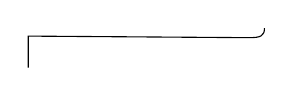
\begin{tikzpicture}\draw (0,0)--(0,0.4)--(2.8,0.38)..controls (2.95,0.38) and (3,0.4)..(3,0.5);\end{tikzpicture}}
\mspage{284}

\scanpage{286}
également un ``bon'' sous-schéma abélien.

\margin{$\unsure{\rho}$}
[N.B. \unsure{Il n'était} pas nécessaire dans \deleted{\illegible{1}} l'exemple plus général que $B$ soit un schéma abélien sur lequel $\Gamma$ opère \deleted{par}\inserted{par} translations.
En effet, en vertu de résultats généraux, on a une suite exacte
\diagram{\begin{tikzcd}[column sep=small]
0\arrow[r]&\deleted{\unsure{A'}}\inserted{\uuline{\operatorname{Pic}}_{A/S}}\arrow[r]&\uuline{\operatorname{Hom}}_S(B,\deleted{\unsure{A'}}\inserted{\uuline{\operatorname{Pic}}_{A/S}})\arrow[r]&\uuline{\operatorname{Hom}}_{S-\mathrm{gr}}(A,\uline{\operatorname{Pic}}_{B/S}^{\tau})\arrow[r]&0
\end{tikzcd}}
\margin{morphismes constants}
\margin{[correspond aux \unsure{bi-inversibles} sur $A\times B$]}
\margin{\unsure{sous les} conditions habituelles sur $B$\ldots}
d'où une suite exacte
\diagram{\begin{tikzcd}[column sep=small]
0\arrow[r]&\uuline{\operatorname{Pic}}_{A/S}^{\Gamma}\arrow[r]&\uuline{\operatorname{Hom}}_{S,\Gamma}(B,\uuline{\operatorname{Pic}}_{A/S})\arrow[r]&\uuline{\operatorname{Hom}}_{S-\mathrm{gr}}(A,\uuline{\operatorname{Pic}}_{B/S}^{\tau})^{\Gamma}
\end{tikzcd}}
Or \deleted{\unsure{tout}} supposons que $A_{\Gamma}=0$ \unsure{ensemblist!} \inserted{et $\Gamma$ \uline{opère trivial!} sur $\uline{\operatorname{Pic}}_{B/S}^{\tau}$}, alors
\[
\uuline{\operatorname{Hom}}_{S-\mathrm{gr}}(A,\uuline{\operatorname{Pic}}_{B/S}^{\tau})^{\Gamma}=0
\]
[utiliser le fait que c'est un schéma non ramifié sur $S$], et il vient
\[
\uuline{\operatorname{Pic}}_{A/S}^{\Gamma}\simeq\uuline{\operatorname{Hom}}_{S,\Gamma}(B,\uuline{\operatorname{Pic}}_{A/S}))
\]
Donc on aura
\[
\text{\textcircled{$*$}}\quad\left\{\begin{array}{l}
\uuline{\operatorname{Pic}}_{X/S}\simeq\uuline{\operatorname{Pic}}_{Y/S}\times\uuline{\operatorname{Pic}}_{A/S}^{\Gamma}\\[1.5em]
\text{d'où}\quad\uuline{\operatorname{Pic}}_{X/S}^{\tau}\simeq\uuline{\operatorname{Pic}}_{Y/S}^{\tau}\times A'^{\Gamma}
\end{array}\right.
\]
\deleted{]}
On peut remarquer qu'on peut supposer de \unsure{$=$}, au lieu que $A$ soit un schéma abélien, que $\operatorname{Alb}(A)$ existe, et $(\operatorname{Alb}(\unsure{M|A}))_{\Gamma}=0$ ensemblistiquement --.
]
\figure{\begin{tikzpicture}[x=1cm,y=1cm]
\draw (0,1.7)..controls (0.2,1.5) and (0.8,1.95)..(0.9,1.57)..controls (1.2,1.8) and (1.6,1.64)..(2,1.8);
\draw (0,0.7)..controls (-0.2,0.55) and (-0.2,0.4)..(0.1,0.35)--(2.5,0.3)--(2.55,0)..controls (2.6,0.38) and (2.65,0.3)..(3.2,0.3);
\end{tikzpicture}}
\mspage{285}

\scanpage{287}
Calcul du $\unsure{p_*|f_*}(\uline{\Omega}^1_{X/S})$. On aura
\margin{\diagram{\begin{tikzcd}[column sep=small]
X\arrow[d,"p"']&A\times_S B\arrow[l,"\Gamma"']\arrow[dl,"q"]\\S&
\end{tikzcd}}}
\[
p_*(\uline{\Omega}^1_{X/S})=q_*(\uline{\Omega}^1_{A\times_S B})^{\Gamma}=\pi_{A*}(\uline{\Omega}^1_{A/S})^{\Gamma}\times\pi_{B*}(\uline{\Omega}^1_{B/S})^{\Gamma}
\]
Donc dans le cas \unsure{plus|précis} où $A$ et $B$ sont des schémas abéliens, \deleted{on trouve} $\Gamma$ opère sur $B$ par translations, on trouve
\[
\text{a)}\quad\deleted{\unsure{p_*}}\quad\omega^1_{X/S}\simeq\omega^1_{B/S}\times(\omega^1_{A/S})^{\Gamma}
\]
Si $S$ est le spectre d'un corps $k$, pour comparer $\operatorname{rang}_k H^1(X,\mathcal O_X)$ et $\operatorname{rang}_k H^0(X,\Omega^1_{X/k})$, on note \deleted{doit} que en vertu de \unsure{$(*)$} on aura
\[
\begin{array}{ll}
\text{a')} &H^0(X,\uline{\Omega}^1_X)\simeq H^0(B,\Omega^1_B)\times H^0(A,\Omega^1_A)^{\Gamma}\\[1em]
\text{b)} &H^1(X,\mathcal O_X)\simeq H^1(Y,\uline{\mathcal O}_Y)\times\underbrace{H^1(A,\uline{\mathcal O}_A)^{\Gamma}}_{t_{A'}^{\Gamma}}
\end{array}
\]
donc comparant avec a), on aura
\[
\operatorname{rang}H^1(X,\mathcal O_X)-\operatorname{rang}\unsure{H^0(X/k,\Omega^1_{X/k})}=\dim t_{A'}^{\Gamma}-\dim(t_A)'^{\Gamma}
\]
Nous voulons donner des exemples où cette \inserted{différence de} dimensions est $>0$, ou $<0$, \deleted{\unsure{enfin}} ou [dans le cas d'une famille] \deleted{chaque}\inserted{les} termes \deleted{\unsure{de cette}} $\dim(t_{A'})^{\Gamma}$ et $\dim(t_A)'^{\Gamma}=\deleted{\unsure{\operatorname{cor}}}\inserted{\dim}(t_A)_{\Gamma}$ varient d'une \unsure{valeur du paramètre} à l'autre \deleted{[\unsure{par un}} [l'une \unsure{spécialisant} l'autre],
\figure{\begin{tikzpicture}\draw (0,0)--(0,0.35)--(1.35,0.35)--(1.38,0.46);\end{tikzpicture}}
\mspage{286}

\scanpage{288}
où $A'^{\Gamma}$ n'est pas plat sur $S$, enfin où il n'y a pas de ``bon'' sous-schéma abélien de $A'^{\Gamma}$. Comme conséquence, on aura des exemples où 1$^\circ$) la symétrie est fausse pour $X$ en l'une ou l'autre direction 2$^\circ$) le \unsure{th} de continuité est faux pour $H^0(X,\Omega^1_X)$ et pour $H^1(X,\uline{\mathcal O}_X)$ 3$^\circ$) $\uline{\operatorname{Pic}}_{X/S}^{\tau}$ n'est pas plat sur $S$ 4$^\circ$) Il n'y a pas de ``bon'' sous-schéma abélien de $\uline{\operatorname{Pic}}_{X/S}^{\tau}$ en particulier «la formation de Pic variété n'est pas compatible avec la spécialisation».
\mspage{287}

\scanpage{289}
Soit $Y=\operatorname{Spec}(V)$, $V$ anneau de valuation discrète

$X$ schéma abélien sur $Y$

$y_0,y_1$ pt fermé resp. gén. de $Y$

$X_0,X_1$ les deux fibres de $X$ \ldots

$F,G$ deux sous-groupes de $X$, \uline{finis} sur $Y$,
\[
\begin{array}{ll}
\unsure{a)|i)}&F_1\not\subset G_1\deleted{\unsure{\ne 0}}\\
\unsure{a')|ii)}&F_0\subset G_0\ne 0\\
\deleted{\unsure{a'')}}\inserted{\unsure{iii)|a'')}}&pF_{\unsure{1|0}}=G_1\qquad(p=\operatorname{car}k(V))
\end{array}
\]
\[
\begin{array}{l}A=X/F\\B=X/G\end{array}
\]
\diagram{\begin{tikzcd}[row sep=small]X\arrow[r,"\alpha"]&A\\X\arrow[r,"\beta"]&B\end{tikzcd}}
hom can.

Considérons $\beta:X\longrightarrow X/G$ (canonique) alors $p\beta$ s'annule sur \deleted{$pX$, donc sur} $F$ \inserted{en vertu de (iii)}, donc se factorise par \uline{$u$}: $X/F-X/G$
\diagram{\begin{tikzcd}[column sep=small]
&X\arrow[dl,"\alpha"']\arrow[dr,"p\beta"]&\\
A\arrow[rr,"u"]&&B
\end{tikzcd}}
\deleted{Cependant} $u_1\notin p\operatorname{Hom}(A_1,B_1)$, en \deleted{\illegible{1}} se plaçant dans $\operatorname{Hom}(X_1,X_1)\otimes\mathbb Q\simeq\operatorname{Hom}(A_1,B_1)\otimes\mathbb Q$, si on avait $u=pv$, on aurait $v=\delta$, or $\delta$ ne provient pas d'un élément de $\operatorname{Hom}(A_1,B_1)$, puisque $F_1\not\subset G_1$ \deleted{[\unsure{sinon}, par (i), on aurait $F_1=0$ d'où $F_0=0$ qui contredit (ii)]}. Cependant $u_0\in p\operatorname{Hom}(A_0,\unsure{F_0|B_0})$, puisque $F_0\subset G_0$.

Les conditions dites (i)(ii)(iii) peuvent être réalisées, en égales ou inégales car, avec pour $X$ une \uline{courbe elliptique}, on prend $X_0$ sans pt d'ordre $p$, $X_1$ avec pt d'ordre $p$, et $F_1$ et $G_1$ deux ss-groupes de $X_1$, \deleted{annulés par $p$}\inserted{de \deleted{\unsure{ordre}} rang $p$ sur $k(y_1)$ et} distincts. Comme il n'y a
\figure{\begin{tikzpicture}\draw (0,1.1)--(0,1.3)--(1.9,1.45)--(1.92,1.55);\draw (0.1,0)--(0.1,0.33)--(2.6,0.31)--(2.7,0.1);\end{tikzpicture}}
\mspage{288}

\scanpage{290}
qu'un seul sous-groupe \inserted{\unsure{fini}} de ${}_pX_0$ de rang $p$ sur $k(y_0)$, on aura $F_0=G_0$, \unsure{d'acc.|d'accord} que $F_1\subset G_1$, et $pF=0\subset G$.

$A$ et $B$ étant comme dessus, considérons,
\[
C=A\times B'\qquad B'\text{ dual de }B
\]
et
\[
\uline{\operatorname{NS}}\deleted{\unsure{(}}_{C/Y}\deleted{\unsure{)}}\simeq\uline{\operatorname{NS}}_{A/Y}\times\uline{\operatorname{NS}}_{B/Y}\times\uline{\operatorname{Hom}}_{Y-\mathrm{gr}}(A,B).
\]
Mais $u$ correspond à une section $\bar u$ de $\uline{\operatorname{NS}}_{C/Y}$ [dont les premières deux composantes sont nulles], et sur la fibre \deleted{\unsure{géné|générique}} spéciale, on a $\bar u_0=p\bar v_0$, mais on ne peut avoir $\bar u=p\bar v$ car alors $\bar v$ nécessairement aurait ses deux premières composantes nulles, donc proviendrait d'une section $v$ de $\uline{\operatorname{Hom}}_{Y-\mathrm{gr}}(A,B)$, on a vu que ce n'était pas possible\ldots
\mspage{289}

\scanpage{291}
\uline{Structure de certains groupes divisibles}.

\deleted{\unsure{Les}} Les groupes de torsion divisibles $\unsure{\mathfrak M|M}$ sont comme l'on sait isomorphes à des sommes directes de groupes $\mathbb Q_p/\mathbb Z_p$ ($p$ premiers); Ceux qui sont $p$-primaires sont donc isom. à des \deleted{sommes directes de} groupes $(\mathbb Q_p/\mathbb Z_p)^{(I)}$, où le cardinal de $I$ est bien déterminé; c'est aussi la dimension de l'espace vectoriel sur $\unsure{p}$ ${}_p\mathfrak M=\operatorname{Hom}(\mathbb Z/p\mathbb Z,\mathfrak M)$.
\deleted{\unsure{Les $\mathfrak M$ en question} de torsion $p$-primaires sont d'ailleurs isomorphes}

Les conditions équivalentes

(i) $\mathfrak M$ groupe de torsion $p$-primaire, et ${}_p\mathfrak M$ est fini

(ii) $\mathfrak M$ isomorphe à un sous-groupe d'un $(\mathbb Q_p/\mathbb Z_p)^{\unsure{n}}$, \deleted{\unsure{$n\in\mathbb Z$}} $n$ entier $\geq0$.

(iii) $\mathfrak M$ isomorphe à un groupe $F+(\mathbb Q_p/\mathbb Z_p)^{\rho}$, où $F$ est un $p$-groupe de torsion fini, et $\rho$ un entier fini.
\margin{Modules sur un anneau de Dedekind.}
Sous ces conditions, $\rho$ est défini de façon unique [c'est aussi $\operatorname{rang}_{\mathbb Z/p\mathbb Z}{}_p\mathfrak M^0$, où $\mathfrak M^0$ est le plus grand sous-groupe divisible de $\mathfrak M$] ainsi que la structure de $F$ [c'est $\mathfrak M/\mathfrak M^0$].

On peut de deux façons différentes faire correspondre à $\mathfrak M$ un module de type fini sur $\mathbb Z_p$:
On peut poser
\[
T_p(\mathfrak M)=\operatorname{Hom}(\mathfrak M,\mathbb Q_p/\mathbb Z_p)=\varprojlim_n\operatorname{Hom}({}_{p^n}\mathfrak M,\mathbb Q_p/\mathbb Z_p)
\]
\margin{$T_p$ \uline{foncteur} \uline{contravariant} en $M$}
[$\mathfrak M\mapsto T_p(\mathfrak M)$ établit une \inserted{anti-}équivalence de la catégorie des $\mathfrak M$ satisfaisant (i), et des modules de type fini sur $\mathbb Z_p$.

On peut prendre aussi
\[
T^p(M)=\varprojlim {}_{p^n}M
\]
\margin{$T^p$ foncteur \uline{covariant} en $M$}
où pour $m\geq n$, on envoie ${}_{p^m}M$ dans ${}_{p^n}M$ par $p^{m-n}$.
\figure{\begin{tikzpicture}\draw (0,0)..controls (0.7,-0.08) and (1.5,0.05)..(2.1,0.09)..controls (2.4,0.1) and (2.25,0.65)..(2.4,0.68)--(4.1,0.67);\end{tikzpicture}}
\mspage{290}

\scanpage{292}
On a un isom canonique
\[
T^p(M)=\operatorname{Hom}(T_p(M),\mathbb Z_p)
\]
On notera que a) $T^p$ n'est pas un foncteur exact, mais seulement exact ``mod groupes finis'' b) $T^p$ s'annule sur tous les groupes finis exactement c) De façon précise, $T^p$ établit une \deleted{\unsure{anti-}}\unsure{équiv.} des catégories ``\uline{mod} les groupes finis'', i.e. essentiellement des \unsure{catégories} avec les espaces vecteurs de dim finie sur $\mathbb Q_p$.

Soit $M\longrightarrow N$ un hom de groupes de la forme $\mathbb Q_p/\mathbb Z_p^{\unsure{n}}$, et $H$ un $p$-groupe fini. \uline{Conditions équivalentes}

(i) $T_p(N)\longrightarrow T_p(M)$ injectif à conoyau libre [i.e. isom sur un facteur]

(i bis) $T_p(N)\otimes H\longrightarrow T_p(M)\otimes H$ injectif

(i ter) \deleted{\unsure{$T_p(M)$}}, $T_p(N)/pT_p(N)\longrightarrow T_p(M)/pT_p(M)$ injectif

(ii) $T^p(M)\longrightarrow T^p(N)$ surjectif

(iii) $M\longrightarrow N$ \unsure{épim} sur un quotient facteur direct

(iv) ${}_pM\longrightarrow {}_pN$ est \uline{surjectif}
\mspage{291}

\scanpage{294}
\margin{\figure{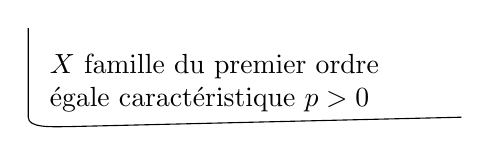
\begin{tikzpicture}\node[align=left,anchor=west] at (0.15,0.55) {$X$ famille du premier ordre\\égale caractéristique $p>0$};\draw (0,1.25)--(0,0.12)..controls (0,-0.02) and (0.3,0)..(0.5,0)--(5.5,0.12);\end{tikzpicture}}}
\diagram{\begin{tikzcd}[column sep=small]
&\uline{\operatorname{Pic}}^{\unsure{00|\infty}}_{X/\unsure{U|S}}\text{ existe}\arrow[d,Leftrightarrow]&&\\
\check V\arrow[r,"\mu"']&H^1(X_0,\unsure{\uline{\mathfrak g}_{X_0}|\uline{\mathcal T}_{X_0}})\arrow[r,"u"']&H^1(X_0,\mathcal O_{X_0})\otimes t_{B_0}\simeq&H^1(X_0,\mathcal O_{X_0})\otimes H^1(A_0,\mathcal O_{A_0})\\
&&&H^1(A_0,\uline{\mathfrak g}_{A_0})\simeq t_{A_0}\otimes H^1(A_0,\uline{\mathcal O}_{A_0})\arrow[u,"v"']
\end{tikzcd}}
\[
\operatorname{Im}u\mu\subset\operatorname{Im}v
\]
\figure{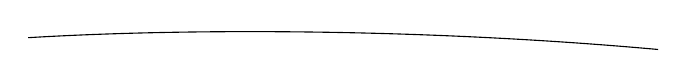
\begin{tikzpicture}\draw (0,0)..controls (2,0.12) and (5,0.12)..(8,-0.15);\end{tikzpicture}}

\diagram{\begin{tikzcd}[column sep=small,row sep=large]
\uline{\operatorname{Pic}}_{X/\unsure{U|S}}\text{ plat sur }S\text{ en }x_0\arrow[d,Rightarrow]&&V\otimes H^{\unsure{2|1}}(X_0,\uline{\mathcal O}_{X_0})\arrow[d,equal]\\
H^1(X_0,\uline{\mathcal O}_{X_0}^{*})\arrow[r,"\partial"']\arrow[dr,"\unsure{d}"']&\operatorname{Hom}(H^1(X_0,\uline{\mathfrak g}_{X_0}),H^{\unsure{2|1}}(X_0,\uline{\mathcal O}_{X_0}))\arrow[r,"\rho"']&\deleted{\operatorname{Hom}}(\check V,H^{\unsure{2|1}}(X_0,\uline{\mathcal O}_{X_0}))\\
&H^1(X_0,\uline{\Omega}^1_{X_0})\arrow[u,"c\ \text{cup}"']&
\end{tikzcd}}
\[
\rho\partial(x)=0\quad\Longleftrightarrow\quad\rho c(x)=0
\]
N.B. Cette condition est automatiquement vérifiée en les pts \inserted{\textcircled{$x_0$}} de $\uline{\operatorname{Pic}}^{\unsure{\sigma|0}}_{X_0/k}\deleted{\unsure{(X_0/k)}}$, mais il est douteux que $\uline{\operatorname{Pic}}^0_{X/k}$ soit pour autant plat sur $S$.
\margin{car $\operatorname{Pic}^0_{X/k}(k)$ est ``divisible par $p$''}
\figure{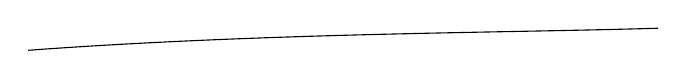
\begin{tikzpicture}\draw (0,0)..controls (3,0.22) and (6,0.22)..(8,0.28);\end{tikzpicture}}
\mspage{293}

\scanpage{295}
- \mspage{11} -
\margin{$n^\circ\ 246$}

similitude amenant $D$ sur $D'$ s'appellera le \uline{diangle} de $D$ et $D'$ et se notera $(D,D')$. Le diangle déterminé par la similitude $S$ est d'ordre $2$ dans le groupe $G_{\unsure{0|o}}/H$. Pour qu'un élément $X=\xi\cdot1_E+\eta S$ de $G_0$ détermine un diangle d'ordre $2$, il faut et il suffit qu'on ait $2\xi\eta=0$ ; donc le diangle déterminé par $S$ est le seul élément d'ordre $2$ dans $G_0/H$ si $k$ n'est pas de caractéristique $2$.

Si $X=\xi\cdot1_E+\eta S$ est un élément de $G_0$, $\xi,\eta$ ne sont pas tous deux nuls; posons $\tau(X)=\eta/\xi$ si $\xi\ne0$, et $\tau(X)=\infty$ si $\xi=0$ ; autrement dit, on pose en tout cas $\tau(X)=\eta/\xi$, le second membre étant entendu au sens du \uline{corps projectif} $k_\infty$ attaché à $k$ (Alg., Chap. II, 2e éd., App. III, $n^\circ\ 5$); Pour que deux éléments $X,X'$ de $G_0$ appartiennent à la même classe suivant $H$, il faut et il suffit que $\tau(X)=\tau(X')$ ; pour qu'un élément $\tau$ de $k_\infty$ soit image par $\tau(X)$ d'un élément de $G_0$, il faut et il suffit qu'on ait $\delta\tau^2\ne1$. Autrement dit, $\tau(X)$ détermine une \uline{bijection} de $G_0/H$ sur le complémentaire dans $k_\infty$ de l'ensemble des racines de $\delta\tau^2=1$ (ensemble à deux éléments si $\delta$ est un carré \unsure{d'ns|dans} $k$, vide dans le cas contraire). On a la formule :
\[
\tau(XX')=\frac{\tau(X)+\tau(X')}{1+\delta\tau(X)\tau(X')}\qquad(9),
\]
dont la vérification est immédiate, d'abord dans le cas où $\tau(X),\tau(X')$, $\tau(XX')$ sont finis, puis dans tous les autres cas.

L'homomorphisme canonique de $G_0$ sur $G_0/H$ induit sur $\Gamma_{\unsure{0|o}}$ un homomorphisme de $\Gamma_0$ dans $G_0/H$ dont le noyau est $\Gamma_0\cap H=\{\pm1_E\}$, groupe à deux éléments si $k$ n'est pas de caractéristique $2$. Mais dans ce cas on peut aussi définir un isomorphisme (non moins \unsure{khânonique|khanonique}) entre ces groupes :

PROPOSITION 2. -- \uline{Pour tout} $X\in G_0$, $N(X)^{-1}X^2$ \uline{est une rotation} ;
\mspage{294}

\scanpage{296}
- \mspage{2} -

\uline{il existe une suite spectrale de $\Lambda$-modules aboutissant à}
$\operatorname{Ext}_{\Lambda}^{*}(\varinjlim A_{\alpha},B)$, \uline{et dont le premier terme est donné par}
\[
E_2^{pq}=\varprojlim_{\alpha}^{(p)}\operatorname{Ext}_{\Lambda}^{q}(A_{\alpha},B).
\]

Utilisons maintenant cette proposition avec $B=\Lambda$ (régulier) et $A_{\alpha}=\operatorname{Ext}_{\Lambda}^{k}(L_k(M_{\alpha}),\Lambda)$. Nous obtenons $E_2^{pq}=0$, $q<k$;
$E_2^{pk}=\varprojlim^{(p)}L_k(L_k(M_{\alpha}))=\varprojlim^{(p)}L_k(M_{\alpha})$ et $E_2^{pq}=0$, $p>\dim\Lambda-q-2$, $q>k$, en vertu du théorème 1, resp. $\alpha)$, $\eta)$, $\vartheta)$ de $(^{1})$ et à cause de l'hypothèse de récurrence. Donc la suite spectrale dégénère en l'isomorphisme
\[
\varprojlim^{(p)}L_k(M_{\alpha})=\operatorname{Ext}_{\Lambda}^{p+k}(\varinjlim\operatorname{Ext}_{\Lambda}^{k}(L_k(M_{\alpha}),\Lambda),\Lambda)\quad\text{pour }p\geq\dim\Lambda-k;
\]
et le \deleted{\unsure{$2^e$}} deuxième membre est bien zéro pour $p>\dim\Lambda-k$, ce qui achève l'induction et la démonstration du théorème 2.

REMARQUE 1. - Le théorème 2, restreint au cas $\Lambda=\mathbb Z$, généralise un résultat de Milnor ($(^{2})$, Appendix).

REMARQUE 2. - Le théorème 2 n'est pas valable en général si I n'est pas filtrant, ou si les $M_{\alpha}$ ne sont pas de type fini.

En ce qui concerne les $\varprojlim^{(i)}M_{\alpha}$ avec $i\leq\dim\Lambda$, nous n'avons que des résultats fragmentaires. A l'aide des méthodes de $(^{2})$, on démontre facilement

\margin{\uline{\unsure{Non filtré ?}}}
PROPOSITION 2. - \uline{Soit} A \uline{un $\Lambda$-module} ($\Lambda$ commutatif) \uline{et} $(M_{\alpha})$ \uline{un système projectif de $\Lambda$-modules. Alors il existe deux suites spectrales} de $\Lambda$-modules \uline{aboutissant à la même limite} $H^{*}$, \uline{avec comme premiers termes}
\[
E_2^{pq}=\varprojlim^{(p)}\operatorname{Ext}_{\Lambda}^{q}(A,M_{\alpha})\quad\uline{\text{et}}\quad {}'E_2^{pq}=\operatorname{Ext}_{\Lambda}^{p}(A,\varprojlim^{(q)}M_{\alpha}).
\]

Soit maintenant $\Lambda$ régulier, I filtrant et les $M_{\alpha}$ et A de type fini. Alors $E_2^{pq}=0$ pour $p>\dim\Lambda-q$ [théorème 1, $\delta)$ de $(^{1})$ et théorème 2], d'où $H^s=0$ pour $s>\dim\Lambda$. La deuxième suite spectrale donne $\operatorname{Ext}_{\Lambda}^{1}(A,\varprojlim^{(1)}M_{\alpha})=0$, si $\dim\Lambda=1$, et $\operatorname{Ext}_{\Lambda}^{\nu-1}(A,\varprojlim^{(\nu)}M_{\alpha})=0$, si $\nu=\dim\Lambda>1$, pour tout $\Lambda$-module A de \uline{type fini}. Mais ceci
\margin{\figure{\begin{tikzpicture}\draw (0,0.12)--(0.04,0)--(0.14,0.24);\end{tikzpicture}}}
\mspage{295}

\scanpage{297}
\diagram{\begin{tikzcd}[column sep=large,row sep=large]
\uline{\operatorname{Pic}}_Y^\tau\simeq\widehat A_1\times\widehat B^{\unsure{\Gamma|\sigma}} \arrow[d,"k"] & {} \\
H^1(Y,\mathcal O_Y)\simeq\underbrace{H^1(A_1,\mathcal O_{A_1})}\times H^1(B,\mathcal O_B)\simeq t_{\widehat A_1}\times t_{\widehat B_{\unsure{\Gamma|\sigma}}}
\arrow[ur,bend left=30] \arrow[d,"{\deleted{\unsure{\text{nul sur le facteur}}}\;\deleted{\unsure{t_B}}}"] & \\
H^1(X,\mathcal O_X)\simeq H^1(A,\mathcal O_A)\times H^1(B,\mathcal O_B) &
\end{tikzcd}}
\figure{\begin{tikzpicture}\draw (0,0) .. controls (1,.1) and (2,-.2) .. (2.5,.1) .. controls (3,.5) and (2.9,.6) .. (3.3,.6) -- (4,.6);\end{tikzpicture}}

\diagram{\begin{tikzcd}[row sep=tiny]
|[draw,ellipse]|\bigl(\underbrace{H^1(B,\mathcal O_B)}\otimes t_A\bigr)\\
t_{\widehat B}\arrow[u,phantom,"\rotatebox{90}{$\simeq$}"]
\end{tikzcd}}
\figure{\begin{tikzpicture}\draw (0,.5) .. controls (2,1.2) and (5,2) .. (5.1,1.9) .. controls (5.15,1.8) and (2,.6) .. (.6,0);\end{tikzpicture}}

\diagram{\begin{tikzcd}[column sep=large,row sep=large]
H^1(Y,\unsure{\mathfrak g|\mathcal T}_Y)=\underbrace{H^1(Y,\mathcal O_Y)}_{t_{\widehat A_1}\times t_{\widehat B}}\otimes(t_A\times t_B)
\arrow[r,"{\unsure{\text{nul sur le facteur}}\;\unsure{\text{provenant de }A|\text{provenant de }B}:\,t_B}"]\arrow[d]
& H^1(Y,\mathcal O_Y)\otimes\overset{t_A}{\overset{\Vert}{t_{A_1}}}. & t_{\widehat A_1}\otimes t_{A_1}\arrow[l]\\
H^1(X,\unsure{\mathfrak g|\mathcal T}_X)=H^1(X,\mathcal O_X)\otimes(t_A\times t_B) & &
\end{tikzcd}}
\[
(t_{\widehat A}\times t_{\widehat B})\otimes(t_A\times t_B)
\]
\[
t_{\widehat B}\otimes t_A,\quad t_{\widehat B}\otimes t_B
\]
\diagram{\begin{tikzcd}
\widehat A & \widehat A_1\arrow[l]\\
A\arrow[r]&A_1\\
\widehat A & \widehat A_1\arrow[l]
\end{tikzcd}}
\diagram{\begin{tikzcd}
t_A\otimes t_{\widehat A}\arrow[r,shift right] & t_{A_1}\otimes t_{\widehat A_1}\arrow[l,shift right]
\end{tikzcd}}

\diagram{\begin{tikzcd}[column sep=small,row sep=large]
\cdot\arrow[r]&\mu_2\arrow[r]&\uline{\operatorname{Pic}}_Y^{\unsure{*|\tau}}\arrow[r]&\uline{\operatorname{Pic}}_X^{\unsure{\Gamma|\sigma}}\arrow[r,dash]&\mu_2\\
&&\widehat A_1\times\widehat B_{(2)}&\widehat A_{\unsure{2|1}}\times\widehat B_{(2)}\arrow[u,phantom,"\rotatebox{90}{$\simeq$}"]&\deleted{\unsure{\to\mu_2}}
\end{tikzcd}}
\mspage{296}

\scanpage{298}
\diagram{\begin{tikzcd}[column sep=small]
&X_1\amalg_Y X_2&\\
X_1\arrow[ur]&&X_2\arrow[ul]\\
&Y\arrow[ul,"\varphi_1"]\arrow[ur,"\varphi_2"']&
\end{tikzcd}}
\diagram{\begin{tikzcd}
X_1\amalg_Y X_2\\
X_1\amalg X_2\arrow[u]\arrow[r,dash]&{}\\
Y\arrow[u,shift left]\arrow[u,shift right]
\end{tikzcd}}
\margin{Contre-exemples par \deleted{\unsure{re}} recollement}

$\varphi_i$ immersions

\uline{exemple !}
\[
X_1=X_2=\overbrace{\operatorname{Spec}k[x,y]}^{\deleted{\unsure{X}}}-\text{origine}
\]
\[
\underbrace{\deleted{Y=\operatorname{Spec}k[t]-\text{origine}}}_{\inserted{Z}}=\operatorname{Spec}k[t,t^{-1}]
\]
$\varphi_1$ \unsure{induit} par \deleted{\unsure{$k[t]\to$}} $\deleted{Y}\inserted{Z}\to X$ défini par les équations :
\[
x=\deleted{\unsure{\varphi_1^*x}}t,\quad y=0
\]
\deleted{$\varphi_2\quad\unsure{Z}\to X\quad x=\unsure{1/t}$}

\deleted{$\varphi_2=\varphi_1\psi\quad\unsure{=}\quad\psi$}
\[
x=1/t,\quad y=0
\]
\figure{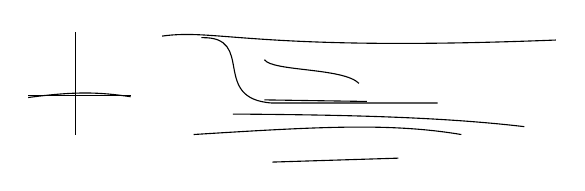
\begin{tikzpicture}[x=1cm,y=1cm]
\draw (0,0)--(1.3,0) (.6,-.5)--(.6,.8);\draw (0,-.03)..controls (.6,.05) and (.9,.04)..(1.3,-.02);
\draw (1.7,.75)..controls (2.4,.85) and (2.9,.55)..(6.7,.7);\draw (2.2,.73)..controls (2.9,.75) and (2.3,-.05)..(3.1,-.1)--(5.2,-.1);
\draw (3,.45)..controls (3.1,.3) and (4,.35)..(4.2,.15);\draw (3,-.06)--(4.3,-.08);
\draw (2.6,-.24)..controls (3.9,-.25) and (5.2,-.27)..(6.3,-.4);\draw (2.1,-.5)..controls (3.7,-.4) and (4.6,-.35)..(5.5,-.5);\draw (3.1,-.85)--(4.7,-.8);
\end{tikzpicture}}

$X'=X_1\amalg X_2$ est \unsure{quasi-affine}.

$X=X_1\amalg_Y X_2$ \unsure{ne l'est pas, car}

$\Gamma(X,\mathcal O_X)=$ \deleted{\unsure{anneau}} \unsure{sous-anneau} de $\Gamma(X')$ formé des $(f_1,f_2)$ telles que
\[
f_1\deleted{\unsure{(t,0)}}\circ\varphi_1=f_2\circ\varphi_2.
\]
Or $\Gamma(X_i,\mathcal O_{X_i})=k[x,y]$, et on a
\[
f_1(t,0)=f_2(1/t,0)
\]
\mspage{297}

\scanpage{299}
- \mspage{3} -
Tribu n$^\circ$ 43

(avec les ``dans le cas séparable c'est déjà connu''. Le sorite du no 2 est assez agréable pour les extensions régulières ; on pourrait donc commencer par celles-ci, et profiter de ce qu'on saura alors pour traiter les extensions primaires.

Chevalley a vendu la démonstration suivante du \uline{lemme de Zariski}. Avec les notations du texte, on suppose $K,E,K(X),E(X)$ plongés dans un domaine universel U (algt. clos) ; soit $u=a(X)/b(X)$ dans $E(X)$, algébrique sur $K(X)$ ; il y a une infinité d'automorphismes s de U sur $K(X)$ ; les éléments $s(u)$ sont en nombre fini ; donc l'ensemble des s tels que $s(u)=u$ est un sous groupe d'indice fini du groupe des $K(X)$-automorphismes de U ; on en déduit que $a(X)=a^{\unsure{s|S}}(X)$ et $b(X)=b^{\unsure{s|S}}(X)$ pour les s de ce sous-groupe, si on a pris la précaution de supposer les polynômes a et b étrangers ; donc a et b ont leurs coefficients algébriques sur K, d'où etcétéra.

Il faut aussi montrer que si K est algébriquement fermé (ou quasi) dans E, et si K' est une extension algébrique finie de K, alors K' est algébriquement fermé (ou quasi) dans E(K'). Voici une démonstration valable en caract. 0, et qu'on pourrait essayer d'arranger : soit K'' la fermeture algébrique de K dans E(K') ; on a $K'\subset K''$ ; or $[E(K'):E]=$ $=[K':K]$ par disjonction linéaire ; de même $[E(K''):E]=[K'':K]$ comme $E(K'')=E(K')$, on en déduit $K''=K'$. C.Q.F.D.

Au n$^\circ$ 4 il faudra expliciter le cas des idéaux principaux (polynômes irréductibles). La remarque d'équidimensionalité ne semble pas plus qu'un exercice. Le fourbi de la p.10 a l'air vrai avec l'hypothèse plus faible que tout élément de S qui est diviseur de 0 dans R l'est dans S (noter que ceci équilibre l'énoncé, qui dit que la propriété se transmet par produit tensoriel).

\mspage{298}

\scanpage{300}
\deleted{\unsure{ce qui exige}} \inserted{\unsure{d'où :}} \deleted{$\unsure{f_1=f_2}$} \inserted{$\unsure{g_1}(t)=\unsure{g_2}(1/t)$} et \uline{$\unsure{g_i}$ est une constante}. Donc les \uline{\unsure{pts} de $Y$ ne sont pas séparés}

On peut aussi \unsure{prendre} un quotient par le groupe $\mathbb Z/2$ [agissant sur $X_1\amalg X_2$ par \unsure{permutation}, et sur $Y$ par $t\mathbin{\unsure{-|\to}}1/t$], on trouve
\margin{\unsure{en réalité ?} \uline{à vérifier}}
\figure{\begin{tikzpicture}\draw (0,.3) .. controls (.5,0) and (.7,.6) .. (1,.3) .. controls (1.5,0) and (1.7,.4) .. (2,.1) .. controls (2.5,-.1) and (3,.15) .. (4,0);\end{tikzpicture}}
\diagram{\begin{tikzcd}
(X_1\amalg_Y X_2)/\mathbb Z_2\\
X_1\amalg X_2\,/\mathbb Z/2\simeq X_1.\arrow[u]
\end{tikzcd}}
\unsure{où|si} $X_1$ est quasi-affine, \deleted{\unsure{comme}} mais non $X_1\amalg_Y X_2\,/\mathbb Z_2$ puisque $X_1\amalg_Y X_2$ le serait \unsure{sinon}.

Il faut cependant vérifier que \unsure{tte} \deleted{partie} \inserted{\unsure{trajectoire}} \deleted{\unsure{trajectoire}} de $X_1\amalg_Y X_2$ par $\mathbb Z/2$ est contenue dans un ouvert affine : c'est facile.
[prendre un \unsure{div} $D$ de $\unsure{\mathfrak X|\mathcal X}$, \inserted{\unsure{contenant le zéro}} \unsure{ne contenant pas} une partie finie, regarder $(\unsure{\mathfrak X|\mathcal X}-D)\amalg(\unsure{\mathfrak X|\mathcal X}-D)$.]
\figure{\begin{tikzpicture}\draw (0,0)--(0,0.4)..controls (0,0.55) and (0.2,0.6)..(0.4,0.58)--(2.5,0.55)..controls (2.6,0.55) and (2.7,0.57)..(2.65,0.68);\end{tikzpicture}}
\mspage{299}

\scanpage{301}
- \mspage{2} -
Tribu 43

invariance du nombre d'éléments de la p-base. Rabiots sur $F^{p^k}$ (cf. bas de la p.22). Ensuite un chapeau disant que, comme toute dérivation de L sur K est nulle sur $K(L^p)$ on est réduit à étudier les dérivations des ext. radicielles (``du premier étage''). La prop.2 ; un cor. disant qu'il existe une dérivation envoyant n'importe où les éléments d'une famille p-indépendante ; donner aussi une condition nécessaire et suffisante pour que les $dx_i$ engendrent.

Le n$^\circ$ 4 (p.23-24) des applications. La prop.4 peut aller en exer. La prop.5 est un bon énoncé ; y nommer a) et b) les deux phrases. . Dans la prop.6, il faut préciser qu'il s'agit de dérivations dans un corps contenant F ; l'énoncer sous forme d'équivalence de : séparabilité, - les dérivations se prolongent, - les différentielles s'injectent.

Il faudra ajouter le sorite à la Lang sur les dimensions d'espaces de dérivations (``le sous truc, la tour, la translation et le compositum'')

\uline{Fabrication d'extensions}.

Ça doit venir à la fin du \S\ sur les extensions cycliques. On exposera la méthode générale (cf. papier que vendra Weil), l'exemple de la théorie de Kummer, celui d'Artin-Schreier simple (cyclique d$^\circ$p), la wittification entre astérisques, et peut être ce qu'on pourra extraire de Klein ou du bouquin de Tchébotarof sur le groupe icosaédrique.

II. - \uline{Matières devant aller en} Alg. \uline{Commutative}, \uline{chapitre des anots affines}.

Une idée du contenu général de ce chapitre est donnée dans les décisions générales. Les choses suivantes proviennent des ``Suppléments'' :

\uline{Extensions régulières et consorts}.

Il s'agit des n$^\circ$2,3,4, du \S1, plus le lemme 2 du n$^\circ$1. Le Congrès objecte au traitement parallèle des ext. régulières, primaires et séparables

\mspage{300}

\scanpage{302}
\uline{Exemple 2} \deleted{Supposons} $X_1=X_2=P^r$, et $\varphi_1,\varphi_2$ sont deux \deleted{\unsure{applications}} immersions \unsure{correspondants} à deux \deleted{\unsure{classes de}} classes $\unsure{\mathcal L_i}$ de $H^1(Y,\uline{\mathcal O}_Y^*)$ \deleted{\unsure{telles que}} qui sont \uline{indépendantes sur $\mathbb Z$} : On peut par exemple supposer $r=2$, $Y$ une courbe elliptique. Alors \deleted{\unsure{un}} tt faisceau inversible sur $X_1\amalg_Y X_2$ est \uline{trivial}, car il induit un faisceau trivial sur $X_1$ \deleted{$\unsure{\times}$}\inserted{et} $X_2$, et l'isom. \unsure{requis} de leurs \deleted{\unsure{restrictions}} images inverses à $Y$, moyennant identifications \uline{convenables} des $\unsure{\uline{L}_i|\mathcal F_i}\unsure{\simeq|:}\uline{\mathcal O}_{X_i}$ $(i=1,2)$ est l'identité. En particulier, $X_1\amalg_Y X_2$ \uline{n'est pas} \uline{projectif}, bien que son normalisé $X_1\amalg_{\deleted{\unsure{Y}}}X_2=\deleted{\unsure{P}}\inserted{P^r\amalg P^r}$ soit.

Ici encore, \deleted{\unsure{faisant opérer} $\mathbb Z/2$} on peut faire un passage au quotient plus compliqué,
\figure{\begin{tikzpicture}\draw[->] (0.4,1.4)--(0.1,1);\draw (1.5,0)--(1.5,0.35)--(2.6,0.4);\end{tikzpicture}}
\mspage{301}

\scanpage{303}
Tribu 43

NOTES SUR LES SUPPLEMENTS DE THEORIE DES CORPS

(Rédaction n$^\circ$ 267, Tribu 43, Marlotte, Octobre 57)

I. - \uline{Matières devant aller en Alg. IV-V}, \uline{2ème édition}.

Le lemme 3, p.12 (Alg.V).

\uline{Suppléments sur les dérivations} (Extraits du \S3).

Le n$^\circ$1 de rappels est inutile.

Le début du n$^\circ$2 (jusqu'à la prop.1 exclue), où on fabrique les différentielles de Kähler, ira au chap.IV. Regarder les rédactions précédentes (projet Koszul de réédition d'Alg.II-III, diplodocus Grothendieck) où le sujet est traité. On dira ``\unsure{diffelles|diffélles} de Kähler'', car on ne sait pas bien quelle est la bonne notion de ``différentielle tout court'' (Dans bien des cas on doit chatrer celles de Kähler). La remarque p.18 mérite mieux qu'une remarque. Vers la l.10 de la p.19, il faut supposer que la base de M est finie. Donner aussi la suite exacte analogue de (1) pour les modules de différentielles.

A partir de la prop.1, ça va au chap.V. Dans la prop.1 on se ramène au cas d'ext. monogènes de 3 types particuliers (cf.n$^\circ$1). Le lemme 1 s'appellera ``lemme d'Audin''. Il y a des fautes de frappe à la p.20 (B et A ont été plusieurs fois intervertis).

Au n$^\circ$ 3, on commence par ne pas parler de dérivations. Notion de famille p-indépendante (linéaire indép. des monômes qu'il faut) ; ça veut dire qu'aucun élément n'est dans le sous corps engendré par les autres. Zornification ; existence de p-bases ; ce sont les familles p-indépendantes qui engendrent l'extension. Pour que la p-base ait d-éléments, il faut et il suffit que le degré de l'extension soit $p^d$ ;

\mspage{302}

\scanpage{304}
\diagram{\begin{tikzcd}[column sep=large,row sep=large]
&X\arrow[d,"p"]\arrow[ddl,"f"']&Y\arrow[l,"i"']\arrow[dl,"pi=\varepsilon fi=q"]\\
&X'\arrow[dl,"f'"]&\\
S\arrow[ur,bend right,"\varepsilon"']&&
\end{tikzcd}}
\margin{$\left\{\begin{array}{l}X\text{ plat sur }S,\text{ et quasi-proj.}\\Y\text{ ss-schéma fermé,}\\\qquad\text{fini et plat sur }S\\X'=X\amalg_Y S\quad(\text{existe }\ldots)\end{array}\right.$}
\diagram{\begin{tikzcd}
0\arrow[r]&\uline{\mathcal O}_X^*\arrow[r]&\unsure{\uline{R}|\uline{\mathcal R}}_{X/S}^*\arrow[r]&\uline{\mathcal D}_{X/S}\arrow[r]&0
\end{tikzcd}}
\deleted{$\unsure{p_*(\uline{\mathcal O}_X^*)}$}
\diagram{\begin{tikzcd}[row sep=large]
0\arrow[r]&p_*(\uline{\mathcal O}_X^*)\arrow[r]&p_*(\uline{R}_{X/S}^*)\arrow[r]&p_*(\uline{\mathcal D}_{X/S})\arrow[r]&0\\
0\arrow[r]&\uline{\mathcal O}_{X'}^*\arrow[r]\arrow[u,"\alpha"]&\uline{R}_{X'/S}^*\arrow[r]\arrow[u,"\beta"]&\uline{\mathcal D}_{X'/S}\arrow[r]\arrow[u,"\unsure{\gamma|\sigma}"]&0
\end{tikzcd}}
\margin{car $R^1p_*(\uline{\mathcal O}_X^*)=0$}

\uline{Lemme}\quad a) $\alpha$ est injectif, et son conoyau s'identifie à
\[
\varepsilon_*(f_*(\uline{\mathcal O}_Y^*)/\uline{\mathcal O}_S^*)=q_*(\uline{\mathcal O}_Y^*)/\varepsilon_*(\uline{\mathcal O}_S^*)
\]
b) $\beta$ est bijectif

\uline{Corollaire 1}\quad $\gamma$ est surjectif, son noyau s'identifie à $\varepsilon_*(f_*\uline{\mathcal O}_Y^*)/\uline{\mathcal O}_S^*)$, d'où une suite exacte de faisceaux sur $X'$ :
\diagram{\begin{tikzcd}
0\arrow[r]&\varepsilon_*(f_*(\uline{\mathcal O}_Y^*)/\uline{\mathcal O}_S^*)\arrow[r]&\uline{\mathcal D}_{X'/S}\arrow[r]&p_*(\uline{\mathcal D}_{X/S})\arrow[r]&0
\end{tikzcd}}

\uline{Corollaire 2}\quad On a une suite exacte de faisceaux sur $S$
\diagram{\begin{tikzcd}
0\arrow[r]&f_*\uline{\mathcal O}_Y^*)/\uline{\mathcal O}_S^*\arrow[r]&f'_*(\uline{\mathcal D}_{X'/S})\arrow[r]&f_*(\uline{\mathcal D}_{X/S})\arrow[r]&0
\end{tikzcd}}

N.B. On a aussi une suite exacte
\diagram{\begin{tikzcd}
0\arrow[r]&f_*\uline{\mathcal O}_Y^*)/\uline{\mathcal O}_S^*\arrow[r]&\unsure{\uline{\mathcal P}|\uline{P}}(X'/S)\arrow[r]&\uline{\mathcal P}(X/S)\arrow[r]&0
\end{tikzcd}}
déduit de la suite exacte
\diagram{\begin{tikzcd}
0\arrow[r]&\uline{\mathcal O}_{X'}^*\arrow[r,"\alpha"]&p_*\uline{\mathcal O}_X^*)\arrow[r]&\varepsilon_*(f_*\uline{\mathcal O}_Y^*)/\uline{\mathcal O}_S^*)\arrow[d]\\
&&&\unsure{0|\cdot}
\end{tikzcd}}
du moins si $f_*\uline{\mathcal O}_X^*)=\uline{\mathcal O}_S^*$
\mspage{303}

\scanpage{305}
Picard et Albanese

pour les variétés non complètes

th. de Chevalley

\mspage{304}

\scanpage{306}
\margin{\deleted{$\unsure{\varphi}$}\quad $\unsure{\xi|6}$}
$X\times Y\longrightarrow Y$ morphisme de schémas algébriques \inserted{(intègres sur $k$ alg clos)}

$D$ diviseur sur $Y$

\uline{Supposons} que pour tt $x\in X(k)$ on ait
\[
\unsure{\varepsilon_x}\; x.D-D\quad\text{lin. équivalent \unsure{à|:}}\quad0
\]
C'est le cas si $X$ \inserted{ou $Y$} est ``d'irrégularité nulle'' et $\exists e\in X$ qui opère trivialement sur $Y$. \deleted{\unsure{C'est bien entendu}}

\deleted{$\unsure{\Rightarrow}$}
\uline{Alors} \deleted{l'ens des $xD$} On peut trouver un \deleted{\unsure{espace projectif} $P$ \unsure{avec famille de dim finie|avec la famille de dim finie}} \deleted{famille linéaire} \inserted{système linéaire} borné $P$ de diviseurs sur $Y$, contenant $D$ et un morphisme $X\times P\longrightarrow P$, qui ensemblistement correspond à : $(x,D)\longrightarrow x.D$.
\figure{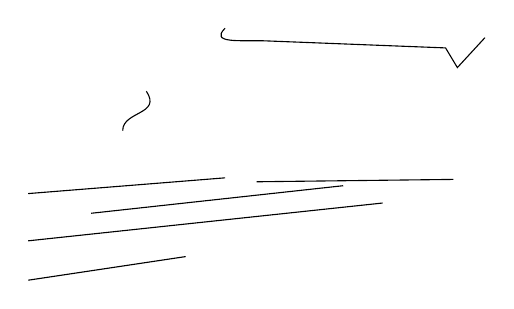
\begin{tikzpicture}[x=1cm,y=1cm]
\draw (2.5,2.6)..controls (2.3,2.4) and (2.7,2.45)..(3,2.44)--(5.3,2.35)--(5.45,2.1)--(5.8,2.48);
\draw (1.2,1.3)..controls (1.2,1.55) and (1.7,1.5)..(1.5,1.8);
\draw (0,.5)--(2.5,.7) (0.8,.25)--(4,.6) (2.9,.65)--(5.4,.68) (0,-.1)--(4.5,.38) (0,-.6)--(2,-.3);
\end{tikzpicture}}
\mspage{305}

\scanpage{307}
ont même fibre générique, il s'ensuit que cette dimension est la même pour $G$ et $H$, donc $u_s:G_s\quad H_{\deleted{\unsure{g}}\inserted{s}}$ est un \uline{monomorphisme} de groupes algébriques \uline{de même dimension}. On en conclut facilement que $G_s$ est ouvert dans $H_s$, et en fait est ensemblistement une \deleted{\unsure{réun}} réunion de composantes connexes de $H_s$ (on est ramené au cas où le corps de base est algébriquement clos, et $G$ et $H$ réduits, donc simples sur $k$, où c'est immédiat ...). Donc $H_s-G_s$ est fermé dans $H_s$, donc dans $H$, donc son complémentaire $H'$ dans $H$ est ouvert, et c'est évidemment un ouvert stable \unsure{pourla|pour la} loi de groupe de $H$. Donc, \deleted{pour prouver que} \deleted{\unsure{$u$ est}} quitte à remplacer $H$ par $H''$, on peut, pour prouver que $u$ est une immersion, se ramener au cas où, en plus des hypothèses précédentes, on suppose $u$ \uline{bijectif}, \deleted{\unsure{en part}} i.e. $u_s:G_s\quad H_s$ \uline{bijectif}. On est donc en tous cas ramené à prouver que $u$ \inserted{ou encore $u_s$} est un isomorphisme, moyennant le cas échéant l'hypothèse de bijectivité.

Supposons donc d'abord que $u$ est bijectif. Si $H_s$ est \uline{réduit}, on peut évidemment conclure que $u_s$ est un isomorphisme, car $G_s$ s'identifie à un sous-schéma fermé de $H_s$ ayant même ensemble sous-jacent. En particulier, si $k=k(s)$ est de caractéristique nulle, tout groupe algébrique sur $k$ est réduit d'après \uline{Cartier}, et on \deleted{\unsure{a la fin}} a ainsi obtenu:

\uline{Proposition} \deleted{\unsure{6|5}}\inserted{7}.2. Soit $u:G\quad H$ un homomorphisme de préschémas en groupes de présentation finie sur $S$. Supposons que $u$ soit un monomorphisme, $G$ plat sur $S$, et les \deleted{caractéristiques}\inserted{corps} résiduel\deleted{\unsure{les}} de $S$ \deleted{\unsure{tou}} de caractéristique nulle. Alors $u$ est uneimmersion.

Lorsque $k(s)$ est de caractéristique $p\quad0$, nous allons nous borner au cas où $G$ \uline{est commutatif}. Alors (avec les réductions faites) $H$ est également commutatif, car c'est l'adhérence schématique de $H_s$, qui
\mspage{306}

\scanpage{308}
\uline{Questions \unsure{ouvertes|ouverts}}
\mspage{307}

\scanpage{309}
Questions sur la structure de $\uline{\mathrm{Pic}}_{X/S}$ \quad ($S$ noeth.)

\margin{O.K. $\Longleftarrow$}
a) $X$ est-il somme \inserted{(disjointe)} de préschémas de type fini sur $S$ ?
\margin{non en général; oui ``géométriquement sur $S$''.}

\margin{$\Longleftarrow$}
\unsure{a'}\deleted{\unsure{b}}) Pour tte partie quasi-compacte $U$ de $X$, est-il vrai que $\overline U$ est q. cpt ? $\Longleftrightarrow$ Pour tt $x\in X$, est-il vrai que $\overline x$ est quasi-compact ?

a'') Est-il vrai que \deleted{\unsure{le schéma}} $\uline{\mathrm{Pic}}^\tau_{X/S}$ est un sous-préschéma \uline{fermé} ?? (Il est en \uline{tous cas \unsure{ouvert}})
\margin{?}

On \unsure{aurait} $a\Rightarrow a'\Rightarrow a''$. La réponse à $a''$ est affirmative si $X$ est \deleted{\unsure{simple}}\inserted{\unsure{normal}} (et \unsure{propre}) sur $S$, mais je ne sais pas pour autant s'il en est de $\unsure{\overline{=}}$ pour $a'$).
\margin{\unsure{l'équiv} au th. de décomposition (résulte du th. d'existence en Géom. formelle); il suffit en \unsure{fait} \unsure{que} un Pic. \unsure{connexe} \unsure{des fibres en soit complet}.}

b) Question: existence du préschéma quotient
\[
\uline{\mathrm{N\acute{e}ron}}^0_{X/S}\inserted{\underset{}{\unsure{\mathrm{NSL}}}}=\uline{\mathrm{Pic}}_{X/S}/\uline{\mathrm{Pic}}^\tau_{X/S}
\]

c) $\uline{\mathrm{Pic}}^\tau_{X/S}$ est-il universellement ouvert sur $S$ ?
\margin{O.K. en les pts \unsure{correspondant} à une torsion de N.S. première à la car. résiduelle}
\margin{\uline{Plat sur $S$} ?}

d) $\uline{\mathrm{Pic}}^\tau_{X/S}$ est-il quasi-compact \inserted{donc de type fini} sur $S$ ?
\margin{\uline{Oui, toujours}}
\margin{(O.K. si $X$ normal sur $S$, \unsure{via} \unsure{un} ``critère d'\unsure{irrégularité|irréductibilité}'' de Weil, à démontrer via \unsure{Géom. formelle} (via lemme Zariski); ? ? ?}
\margin{(OK. si les fibres sont \unsure{primaires|prénormales})}

e) $\uline{\mathrm{Pic}}^\tau_{X/S}$ est-il séparé sur $S$ ?
\margin{\uline{non} si on ne le suppose pas \unsure{représentable}; l'est-il s'il est représentable ?}

\deleted{\unsure{f}}\inserted{\unsure{b'}}) demi-continuité de (\unsure{Min.|Dim.} Lissité) des fibres ....

\margin{$\leftarrow$}
\unsure{f}) Continuité de $\unsure{\ell}$-\unsure{rang} des Picard des fibres
\margin{OK si $X$ normal sur $S$, plus gén. si les \unsure{comp. connexes} de Picard des fibres sont complètes, via groupe fondamental}

g) $\uline{\mathrm{Pic}}^\tau\deleted{\unsure{(X\times_S Y)}}_{X\times Y/S}\simeq\uline{\mathrm{Pic}}^\tau_{X/S}\times_S\uline{\mathrm{Pic}}^\tau_{Y/S}$
\margin{O.K. \deleted{si $X$ et $Y$ sont à fibres \unsure{géom. intègres|géom. connexes} [condition plus ou moins \unsure{nécessaire} vérifier.]}}

h) Si $Y$ section hyperplane de $X$,
\[
\uline{\mathrm{Pic}}^\tau_{X/\unsure{k|u}}\longrightarrow\uline{\mathrm{Pic}}^\tau_{Y/\unsure{k|u}}\quad\text{bijectif ? \unsure{Isom?|Sous?}}
\]
\[
\uline{\mathrm{Pic}}_{X/\unsure{k|u}}\mathbin{\unsure{-|\to}}\uline{\mathrm{Pic}}^{\unsure{\tau|0}}_{Y/\unsure{k|u}}\quad\text{\unsure{surjectif}}
\]
\margin{conditions à préciser....}

\figure{\begin{tikzpicture}[x=1cm,y=1cm]
\draw (0,4) .. controls (-.4,3) and (-.65,1) .. (0,0);
\draw (-.1,4.05) .. controls (0,3.85) and (.12,3.85) .. (.2,4.02);
\draw (0,0) -- (-.05,.3);
\end{tikzpicture}}
\figure{\begin{tikzpicture}[x=1cm,y=1cm]
\draw (0,5.8) .. controls (-.2,6.2) and (1.1,6.4) .. (1.4,6.05) .. controls (1.6,5.75) and (.3,5.55) .. (0,5.8);
\draw (.15,5.72) -- (.1,5.4);
\draw (2.9,4.25) .. controls (2.4,4.45) and (2.6,5.15) .. (3.15,5.12) .. controls (3.8,5.3) and (4.6,4.9) .. (4.85,4.86);
\draw (2.85,4.3) .. controls (3.4,4.05) and (4.3,3.95) .. (4.9,4.05);
\draw (2.82,4.7) .. controls (2.3,4.35) and (2.2,4.1) .. (2.05,3.8);
\draw (0,2.65) .. controls (-.3,3.05) and (1.9,3.1) .. (2.1,2.8) .. controls (2.2,2.45) and (.15,2.4) .. (0,2.65);
\draw (.15,2.5) -- (0,2.28);
\draw (2.75,.1) -- (3.65,2.15);
\draw (3.15,0) -- (4.05,2.05);
\draw (3.7,0) -- (4.5,1.95);
\draw (4.25,.08) -- (4.85,1.6);
\end{tikzpicture}}
\mspage{308}

\scanpage{310}
1) $\uline{\mathrm{Pic}}^\tau$ \uline{fermé} ds $\uline{\mathrm{Pic}}$ ? OK si $f$ est \uline{normal} \deleted{\unsure{universellement} \illegible{1}}

2) $\uline{\mathrm{Pic}}^\tau$ plat sur $S$ ?
\margin{\uline{Non} [contre-exemple de Mumford...]}
\deleted{\unsure{univ. ouvert sur $S$ ?}}

3) $\uline{\mathrm{Pic}}^\tau$ \unsure{univ$^t$} ouvert sur $S$ ?
\margin{\uline{si $f$ normal,} [Vrai, \unsure{en les pts} \deleted{\unsure{dont la}} \inserted{\unsure{de} $\unsure{\tau}$} torsion est première aux car. rés. \unsure{?} OK. en car. $0$]}

4) \deleted{\unsure{4}} La multiplication par $n$ dans $\uline{\mathrm{Pic}}$ (ou dans \deleted{\unsure{$\uline{\mathrm{Pic}}^\tau$ est de type fini}} $\uline{\mathrm{Pic}}^\tau$) est-elle \uline{univ. ouverte} ? (Voir N.b) ?
\inserted{\unsure{pour $n$ ``qcq''}}
\margin{\unsure{expliciter}}
[Oui si $n$ premier aux car. résiduelles; une réponse affirmative à 4), \deleted{pour tt} dans $\uline{\mathrm{Pic}}^\tau$, pour \uuline{tt} $n$, implique une réponse affirmative à 3]
\margin{La multiplication par $n$ est-elle de type fini ?}

\margin{N.B. Soit $G$ un préschéma en groupes sur $S$, tel que les $G_s^\tau$ soient propres, plus gén. \unsure{sans} comp. additives. Alors $G^\tau\to S$ est univ$^t$ ouvert en les pts dont l'ordre de torsion est premier aux car. résiduelles [ $\Longleftarrow$ si $n$ premier aux car. résiduelles, le morphisme $G\xrightarrow{n}G$ est \uuline{étale} ]}

5) $\uline{\mathrm{Pic}}^\tau$ \uline{de type fini sur $S$} $(\Leftrightarrow)$ propre sur $S$
\margin{\uuline{Oui}}
[Si $f$ \deleted{\unsure{normal}}\inserted{\unsure{lisse}}, celà implique $\uline{\mathrm{Pic}}^\tau$ \uline{projectif} sur $S$, j'ignore s'il en est de $\unsure{\overline{=}}$ si $f$ est normal ...]

\unsure{5'}) Une réponse affirmative à 3) en implique une à 5), \deleted{\unsure{dans tous les cas}} \uline{si} $f$ \uline{normal}

OK si les \deleted{$\unsure{\mathrm{NS}}_{\unsure{X_s/k(s)}}$}\inserted{$X_s/k(s)$} ``sans torsion''

\margin{Non, exemple}
\figure{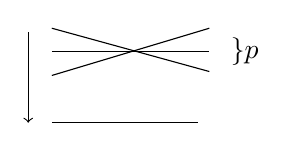
\begin{tikzpicture}[x=1cm,y=1cm]
\draw (0,.65)--(2,.1);\draw (0,.35)--(2,.35);\draw (0,.05)--(2,.65);
\node at (2.45,.35) {$\}p$};
\draw[->](-.3,.6)--(-.3,-.55);\draw (0,-.55)--(1.85,-.55);
\end{tikzpicture}}
\margin{La multiplication par un multiple de $p$ est \unsure{surjective} \illegible{2} \unsure{ouverte} (?) \unsure{comp. irréductibles}}

6) $\uline{\mathrm{Pic}}^\tau$ \deleted{\unsure{est}} n'a-t-il qu'un nb fini de \unsure{$S$-points d'ordre $n$}. \unsure{Non}
\[
[(\uline{\mathrm{Pic}}^\tau_{X/S}\text{ de type fini}\Longleftrightarrow\uline{\mathrm{Pic}}^\tau_{X'/S'}\text{ n'a qu'un nb fini de comp. irréductibles \unsure{au dessus|en dehors} d'un ouvert \unsure{non vide convenable|dense de $S'$ constructible}, }\forall S'\text{ fermé irréductible de }S.
\]

7) $\unsure{\mathrm{rang}}(\mathrm{NS})$ reste-t-il majoré ?
\margin{\uuline{oui}}

8) \deleted{\unsure{$\uline{\mathrm{Pic}}^\tau$ est de type fini sur}}
Les composantes connexes de $\uline{\mathrm{Pic}}_{X/S}$ sont elles de type fini sur $S$ ??
\margin{\uuline{non}}
$\uline{\mathrm{Pic}}_{X/S}$ est-il réunion disjointe \deleted{\unsure{par}}\inserted{de} $\uline{\mathrm{Pic}}^\tau_{X/S}$ ?
\margin{$\unsure{\overline M}$ la réponse à 5) ne semble \unsure{pas aussi évidente ici|pas asymptotiquement liée} .... \unsure{d'invariants} \uline{\unsure{stables|étales}}}

9) Définition de $\uline{\mathrm{Pic}}_{X/k}/\uline{\mathrm{Pic}}^\tau_{X/k}$ ...

\figure{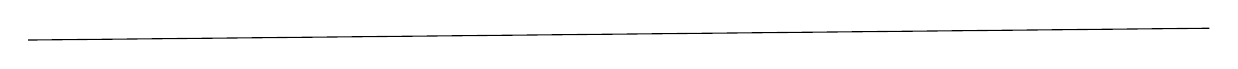
\begin{tikzpicture}\draw (0,0)--(15,.15);\end{tikzpicture}}
\uline{Howard} $\left\{\begin{array}{l}\text{Multiplicité de }\uline{\mathrm{Pic}}^\tau\\ \circledast\ \text{Compatibilité aux spécialisations ???}\end{array}\right.$
\margin{$\circledast$ Questions liées à la \unsure{platitude|flèche}}
\margin{$\circledast$ Questions d'existence et descente....}

\figure{\begin{tikzpicture}[x=1cm,y=1cm]
\draw[->,double] (0,5.3)--(0,4.7);
\draw[<->,double](-.25,4.4)..controls(-.55,3.8)and(-.5,2.8)..(-.25,2.2);
\draw[<->,double](0,1.4)--(0,0);
\draw[->,double](.3,-.35)--(.3,-1.15);
\draw[->](1.5,4.1)..controls(2.2,3.9)and(2.1,1)..(4.1,.9);
\draw[<->](3.4,4.4)--(4.1,4.9);
\end{tikzpicture}}
\figure{\begin{tikzpicture}[x=1cm,y=1cm]
\draw (1.8,8.1) ellipse (.26 and .22);
\draw (1.55,7.99) -- (1.3,7.8);
\draw (.9,6.9) ellipse (.72 and .13);
\draw (-.65,6.45) ellipse (.35 and .18);
\draw[->](-.4,6.7)--(-.7,6.25);
\draw (-1.1,5.3) .. controls (-1.35,5.5) and (-1.1,5.9) .. (-.8,5.95) .. controls (.1,6.2) and (.35,5.55) .. (-.2,5.25) .. controls (-.55,5.05) and (-.9,5.13) .. (-1.1,5.3);
\draw (-.95,4.5) ellipse (.35 and .22);
\draw (2.8,3.15) .. controls (3.7,3.22) and (4.4,3.2) .. (4.9,3.13) -- (5,1.4) .. controls (5.1,.75) and (4.7,.8) .. (4.35,.8) -- (2.65,.84) .. controls (2.25,.9) and (2.3,1.2) .. (2.4,1.6) -- (2.8,3.15);
\draw (4.55,.85) .. controls (4.7,.6) and (5.1,.55) .. (5.18,.82);
\draw (-1.25,.15) ellipse (.3 and .17);
\draw (-1.12,-.55) ellipse (.36 and .2);
\draw (-.85,7.65) .. controls (-.65,7.25) and (-.72,6.9) .. (-.8,6.6);
\draw (-.89,7.67) .. controls (-.7,7.25) and (-.77,6.9) .. (-.85,6.61);
\end{tikzpicture}}
\mspage{309}

\scanpage{311}
$\uline{\mathrm{Pic}}^\tau_{X/S}$ univ$^t$ ouvert sur $S$ ?

$\uline{\mathrm{Pic}}^0_{X/S}$ plat sur $S$ ? \qquad ($\Rightarrow\ \uline{\mathrm{Pic}}^\tau_{X/S}$ plat sur $S$)

Existence de $\uline{\mathrm{Pic}}^{\unsure{00|\infty}}_{X/S}\left\{\begin{array}{l}\text{dans le cas Artinien \unsure{local}}\\\text{dans le cas }S\text{ réduit ???}\end{array}\right.$

\uline{Continuité} de \uline{la torsion de} N.S.

\figure{\begin{tikzpicture}[x=1cm,y=1cm]
\draw (0,0)..controls(4,.2)and(11,.3)..(15,0);
\draw[->](13.5,2)..controls(13.9,2.4)and(13.2,1.7)..(13.55,1.6)..controls(13.5,.5)and(13.35,0)..(12.9,-.7);
\end{tikzpicture}}
\margin{étudier la famille \unsure{modulaire} de la surface de Igusa...}
\mspage{310}

\scanpage{312}
- \mspage{20} -
\margin{n° \unsure{2|1}69}

les de $G'$ et $G'_1$) et que $u_1=f\circ u$.

2) Lorsque $A=B=G$ (la structure de $(A,A)$-bimodule de $A$ étant définie par les homothéties à gauche et à droite), et que $A'=B'$ et $h=h'$ on peut prendre pour $G'$ l'anneau $A'$ et pour $u$ l'homomorphisme $h$ de $A$ dans $A'$.

3) Supposons que l'on ait $A=B$, $A'=B'$, $h=h'$, que les anneaux $A$ et $A'$ soient \uline{commutatifs}, et que la structure de $A$-module à gauche de $G$ coincide avec sa structure de $A$-module à droite. On peut alors prendre pour $G'$ le produit tensoriel $A'\otimes_A G$ (la structure de $A'$-module à droite de $G'$ coincidant avec sa structure de $A'$-module à gauche) et pour $u$ l'application $g\to1\otimes g$ ($g\in G$) de $G$ dans $G'$. Nous dirons alors que la forme bilinéaire (resp. sesquilinéaire) $\Phi'$ définie par la prop. 1 (resp. prop.2) est obtenue à partir de $\Phi$ \uline{par extension de l'anneau de base}, ou \uline{par extension des scalaires}.

Ce qui suit est valable aussi bien dans le cas bilinéaire que dans le cas sesquilinéaire ; les hypothèses et notations sont celles de la prop.1 (resp. prop.2). Etant donné un sous module $M$ de $E$ ou $F$, on désignera par $M'$ le sous module de $E'$ ou $F'$ engendré par l'image canonique de $M$.

PROPOSITION 3 - \uline{Les hypothèses et notations étant celles de la prop.1} (resp. \uline{prop.2}) \uline{supposons de plus que} $A,B,A',B'$ \uline{soient des corps et que les applications} $\alpha$ \uline{et} $\beta$ \uline{de} $A'\otimes_A \uline{G}$ \uline{et} $G\otimes_A B'$ \uline{dans} $G'$ \uline{caractérisées par} $\alpha(a'\otimes g)=a'u(g)$ \uline{et} $\beta(g\otimes b')=u(g)b'$ ($a'\in A'$, $b'\in B'$, $g\in G$) \uline{soient injectives}. \uline{Soient} $M$ \uline{un sous}
\mspage{311}

\scanpage{313}
\uline{Séparation} de $\uline{\mathrm{Pic}}_{X/S}$

(i) Séparé sur $S$ si $X_s$ sont géom$^t$ loc. intègres ?

(ii) $\uline{\mathrm{Pic}}^\tau_{X/S}$ séparé sur $S$ si les $X_s$ séparables ?

${}_n\uline{\mathrm{Pic}}_{X/S}$ \qquad `` \qquad `` \qquad ?

\uline{N.B.} 1) Exemple de Mumford par des ``schémas en courbes elliptiques'', à fibre double, montre que $\uline{\mathrm{Pic}}^0_{X/S}$ peut ne pas être séparé sur $S$.
\margin{(mais alors il n'est pas représentable}

2) Exemple de
\figure{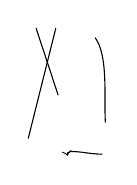
\begin{tikzpicture}[x=1cm,y=1cm]
\draw (0,0)--(.35,1.4);\draw (.1,1.4)--(.38,.55);
\draw (.85,1.28)..controls(1.02,1.05)and(.96,.5)..(.98,.2);
\draw[->](.94,-.2)..controls(.75,-.2)and(.48,-.12)..(.5,-.22);
\end{tikzpicture}}
montre que, $=$ si les fibres sont séparables, $\uline{\mathrm{Pic}}_{X/S}$ n'est pas tjrs \unsure{davantage} séparé sur \unsure{la|$S$}

\uline{Variation de} $\alpha,\lambda,\mu$.

(i) Constance de $\dim\uline{\mathrm{Pic}}_{X_s/k(s)}=\alpha_s+\mu_s+\lambda_s$ ?

(ii) $\alpha\leq\alpha'$, $\lambda\geq\lambda'$, \quad [$2\alpha+\mu\leq2\alpha'+\mu'$ connu]

\margin{du moins pour fibres séparables}

Soient $X,Y$ propres sur $S$, à fibres géom. intègres. Le préschéma. $\uline{\mathrm{Corr}}_S(X,Y)$ [classes de correspondances] existe-t-il ? \uuline{Oui}, par Raynaud ...
\mspage{312}

\scanpage{314}
\uline{Proposition.} Soit $X$ propre, plat, de prés. finie sur $S$. Alors $\uline{\mathrm{Pic}}^\tau_{X/S}$ est un sous-foncteur \uline{ouvert} \inserted{de prés. finie} de $\uline{\mathrm{Pic}}_{X/S}$. L'immersion ouverte $\uline{\mathrm{Pic}}^\tau_{X/S}\to\uline{\mathrm{Pic}}_{X/S}$ est aussi une immersion fermée si $X$ est \inserted{projectif} à fibres géom. intègres.
\margin{projectif est-il nécessaire ? \deleted{\unsure{plt. suffit}} \deleted{\uuline{\unsure{en fait}}}}

Cette assertion équivaut au

\uline{Corollaire.} $X$ comme dessus, $\uline{L}$ un module inversible. Alors l'ens \inserted{$U$} des $s\in S$ tels que $\uline{L}_s$ sur $X_s$ soit \deleted{\unsure{alg}} $\tau$-équiv. à $0$ est \uline{ouvert} \uline{rétrocompact}. Il est ouvert et fermé si $X$ est \inserted{projectif} à fibres géom. intègres.

On peut supposer $S$ noethérien. À prouver que $U$ est stable par générisation, et que si $s\in U$, alors $U\cap\overline{\{s\}}$ \deleted{est un \unsure{ouvert}} contient un ouvert non vide de $\overline{\{s\}}$. Or le critère (viii$'$ b$'$) implique facilement la première condition (en se ramenant au cas où \deleted{$U$ est \unsure{ouvert}} $S$ est un trait, et où son pt fermé $s$ est dans $U$). La deuxième condition est pratiquement triviale. Pour prouver que $U$ est \uline{fermé} si $X/S$ \inserted{projectif} à fibres géom. intègres, on est \deleted{\unsure{encore}} ramené à prouver qu'il est stable par spécialisation. On le voit sur le critère (viii e), \deleted{\unsure{a}}

\uline{Question} Éliminer l'hyp. projective dans la deuxième partie.
Prouver, si $X\to S$ est \uline{normal}, que $\uline{\mathrm{Pic}}^0_{X/S}$ est ``fermé'' dans $\uline{\mathrm{Pic}}_{X/S}$ mieux, que $\uline{\mathrm{Pic}}^0_{X/S}$ est \uline{propre sur $S$} ?? Cela signifie
\margin{?}
\figure{\begin{tikzpicture}\draw(0,0)--(0,1.2);\draw(.08,0)--(.08,1.2);\end{tikzpicture}}
\figure{\begin{tikzpicture}[x=1cm,y=1cm]
\draw[thin] (3.8,6.9)--(3.6,6.5);
\draw (3.3,5.95) .. controls (3.25,6.25) and (3.9,6.25) .. (4,6.35);
\draw (2.5,5.1) .. controls (2.48,5.35) and (2.9,5.34) .. (3.05,5.5);
\draw (.8,3.5) .. controls (.84,3.65) and (1.05,3.75) .. (1,3.9);
\draw (3.3,3.05) .. controls (3.27,3.3) and (3.75,3.3) .. (3.8,3.5);
\draw (.8,.5) .. controls (.8,.7) and (1.3,.7) .. (1.4,.9);
\end{tikzpicture}}
\mspage{313}

\scanpage{315}
aussi: si $X$ est normal et propre sur le \uline{trait} $S$, (avec $f_*(\uline{\mathcal O}_X)=\uline{\mathcal O}_S$ si on veut), et muni d'une section $g$ sur $S$, alors tout module inversible $\uline{L}_t$ sur $\unsure{\uline{X}_t|X_t}$ ($t$ pt générique de $S$), qui est \uline{alg. équiv. à $0$} se prolonge-t-il \inserted{en $\uline{L}$} à $X$ \inserted{et $\uline{L}_s$ est alg. équiv. à $0$} ?? C'est vrai si $\uline{\mathrm{Pic}}_{X/S}$ est représentable, ce qui \deleted{d'après Raynaud} est le cas si $X/S$ est \uline{projectif} ! Peut-être est-ce tjrs le cas \deleted{\illegible{1}} (i.e. $\uline{\mathrm{Pic}}_{X/S}$ représentable si $X\to S$ propre plat et à fibres géom. normales, voire seulement intègres...) ?
\figure{\begin{tikzpicture}[x=1cm,y=1cm]
\draw (0,1.5) .. controls (.12,1.7) and (.25,1.9) .. (.27,2.1);
\draw (1.8,1.3) .. controls (1.65,1.9) and (1.7,1.96) .. (2.25,1.96) -- (4.3,2);
\end{tikzpicture}}
\mspage{314}
